\chapter{Resultados} 
\label{cap5_resultados}

\section{Front-end}

\subsection{Protótipos}

Após a reunião de levantamento de requisitos, protótipos das telas principais da plataforma foram construídos no Figma para validação junto ao setor. Esses protótipos estão disponíveis no repositório do projeto, no endereço \url{https://github.com/Tomaz5556/Horarios-IFNMG-Salinas/blob/main/prototipos/figma.pdf}. A seguir, são apresentadas as telas desenvolvidas:

\begin{figure}[htb]
    \centering
    \caption{Protótipo da tela inicial}
    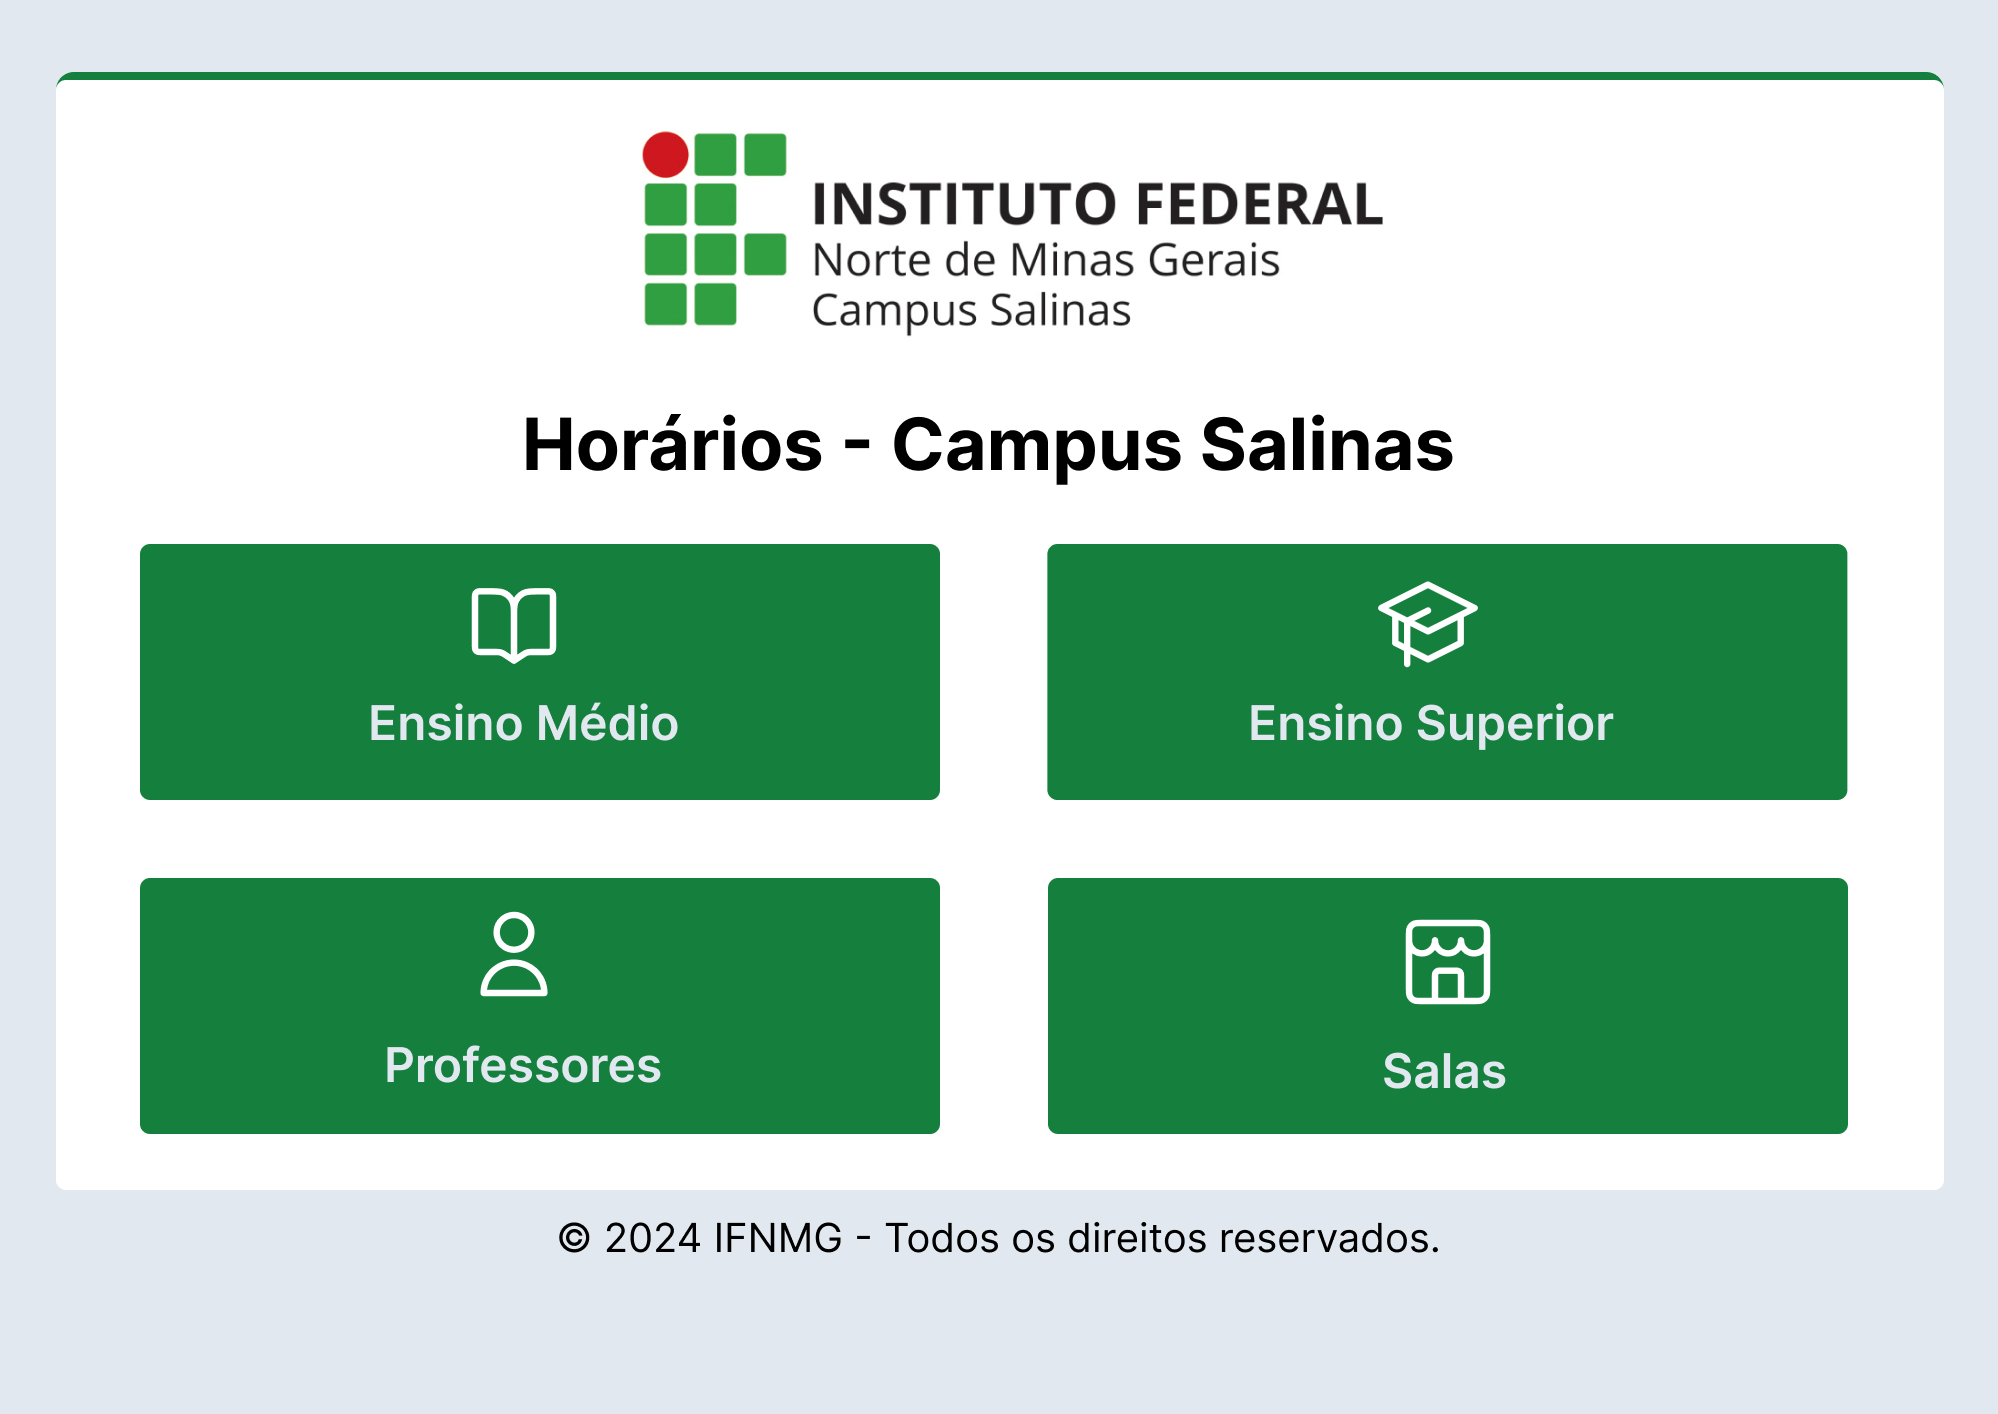
\includegraphics[width=1\textwidth]{Figuras/proto-1.png}
    \caption*{Fonte: AUTOR (2024)}
    \label{fig_proto_1}
\end{figure}

A Figura \ref{fig_proto_1} exibe o protótipo da tela inicial da plataforma, onde o usuário encontra quatro opções para selecionar o tipo de horário.

\begin{figure}[H]
    \centering
    \caption{Protótipo da tela dos cursos}
    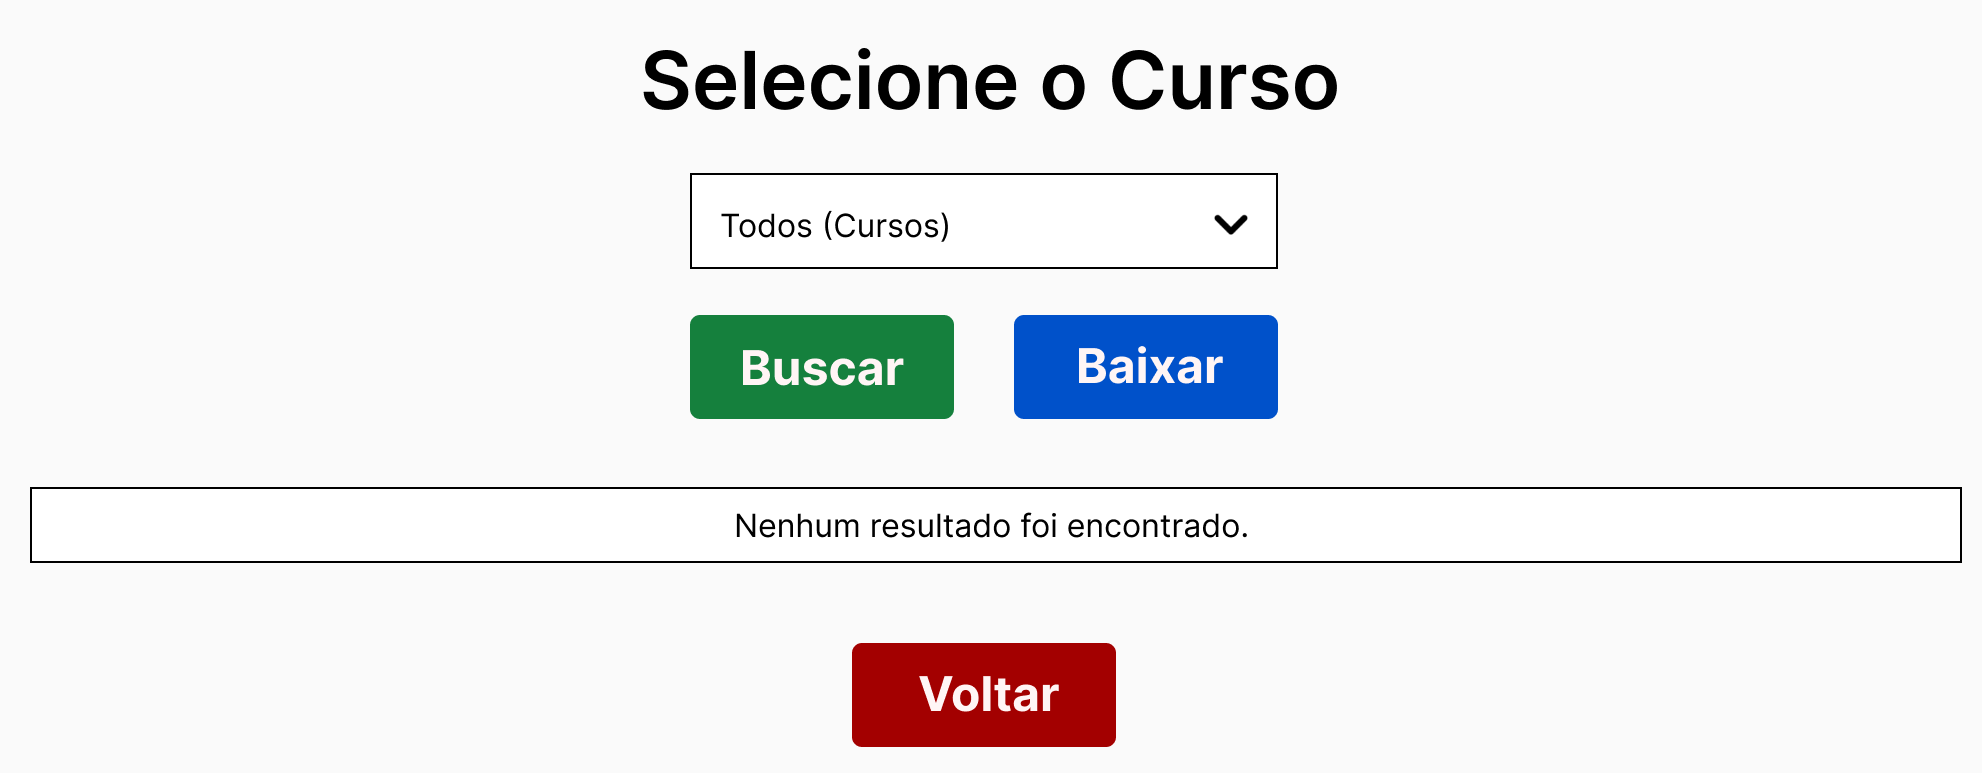
\includegraphics[width=1\textwidth]{Figuras/proto-2.PNG}
    \caption*{Fonte: AUTOR (2024)}
    \label{fig_proto_2}
\end{figure}

\begin{figure}[htb]
    \centering
    \caption{Protótipo da tela dos cursos preenchida}
    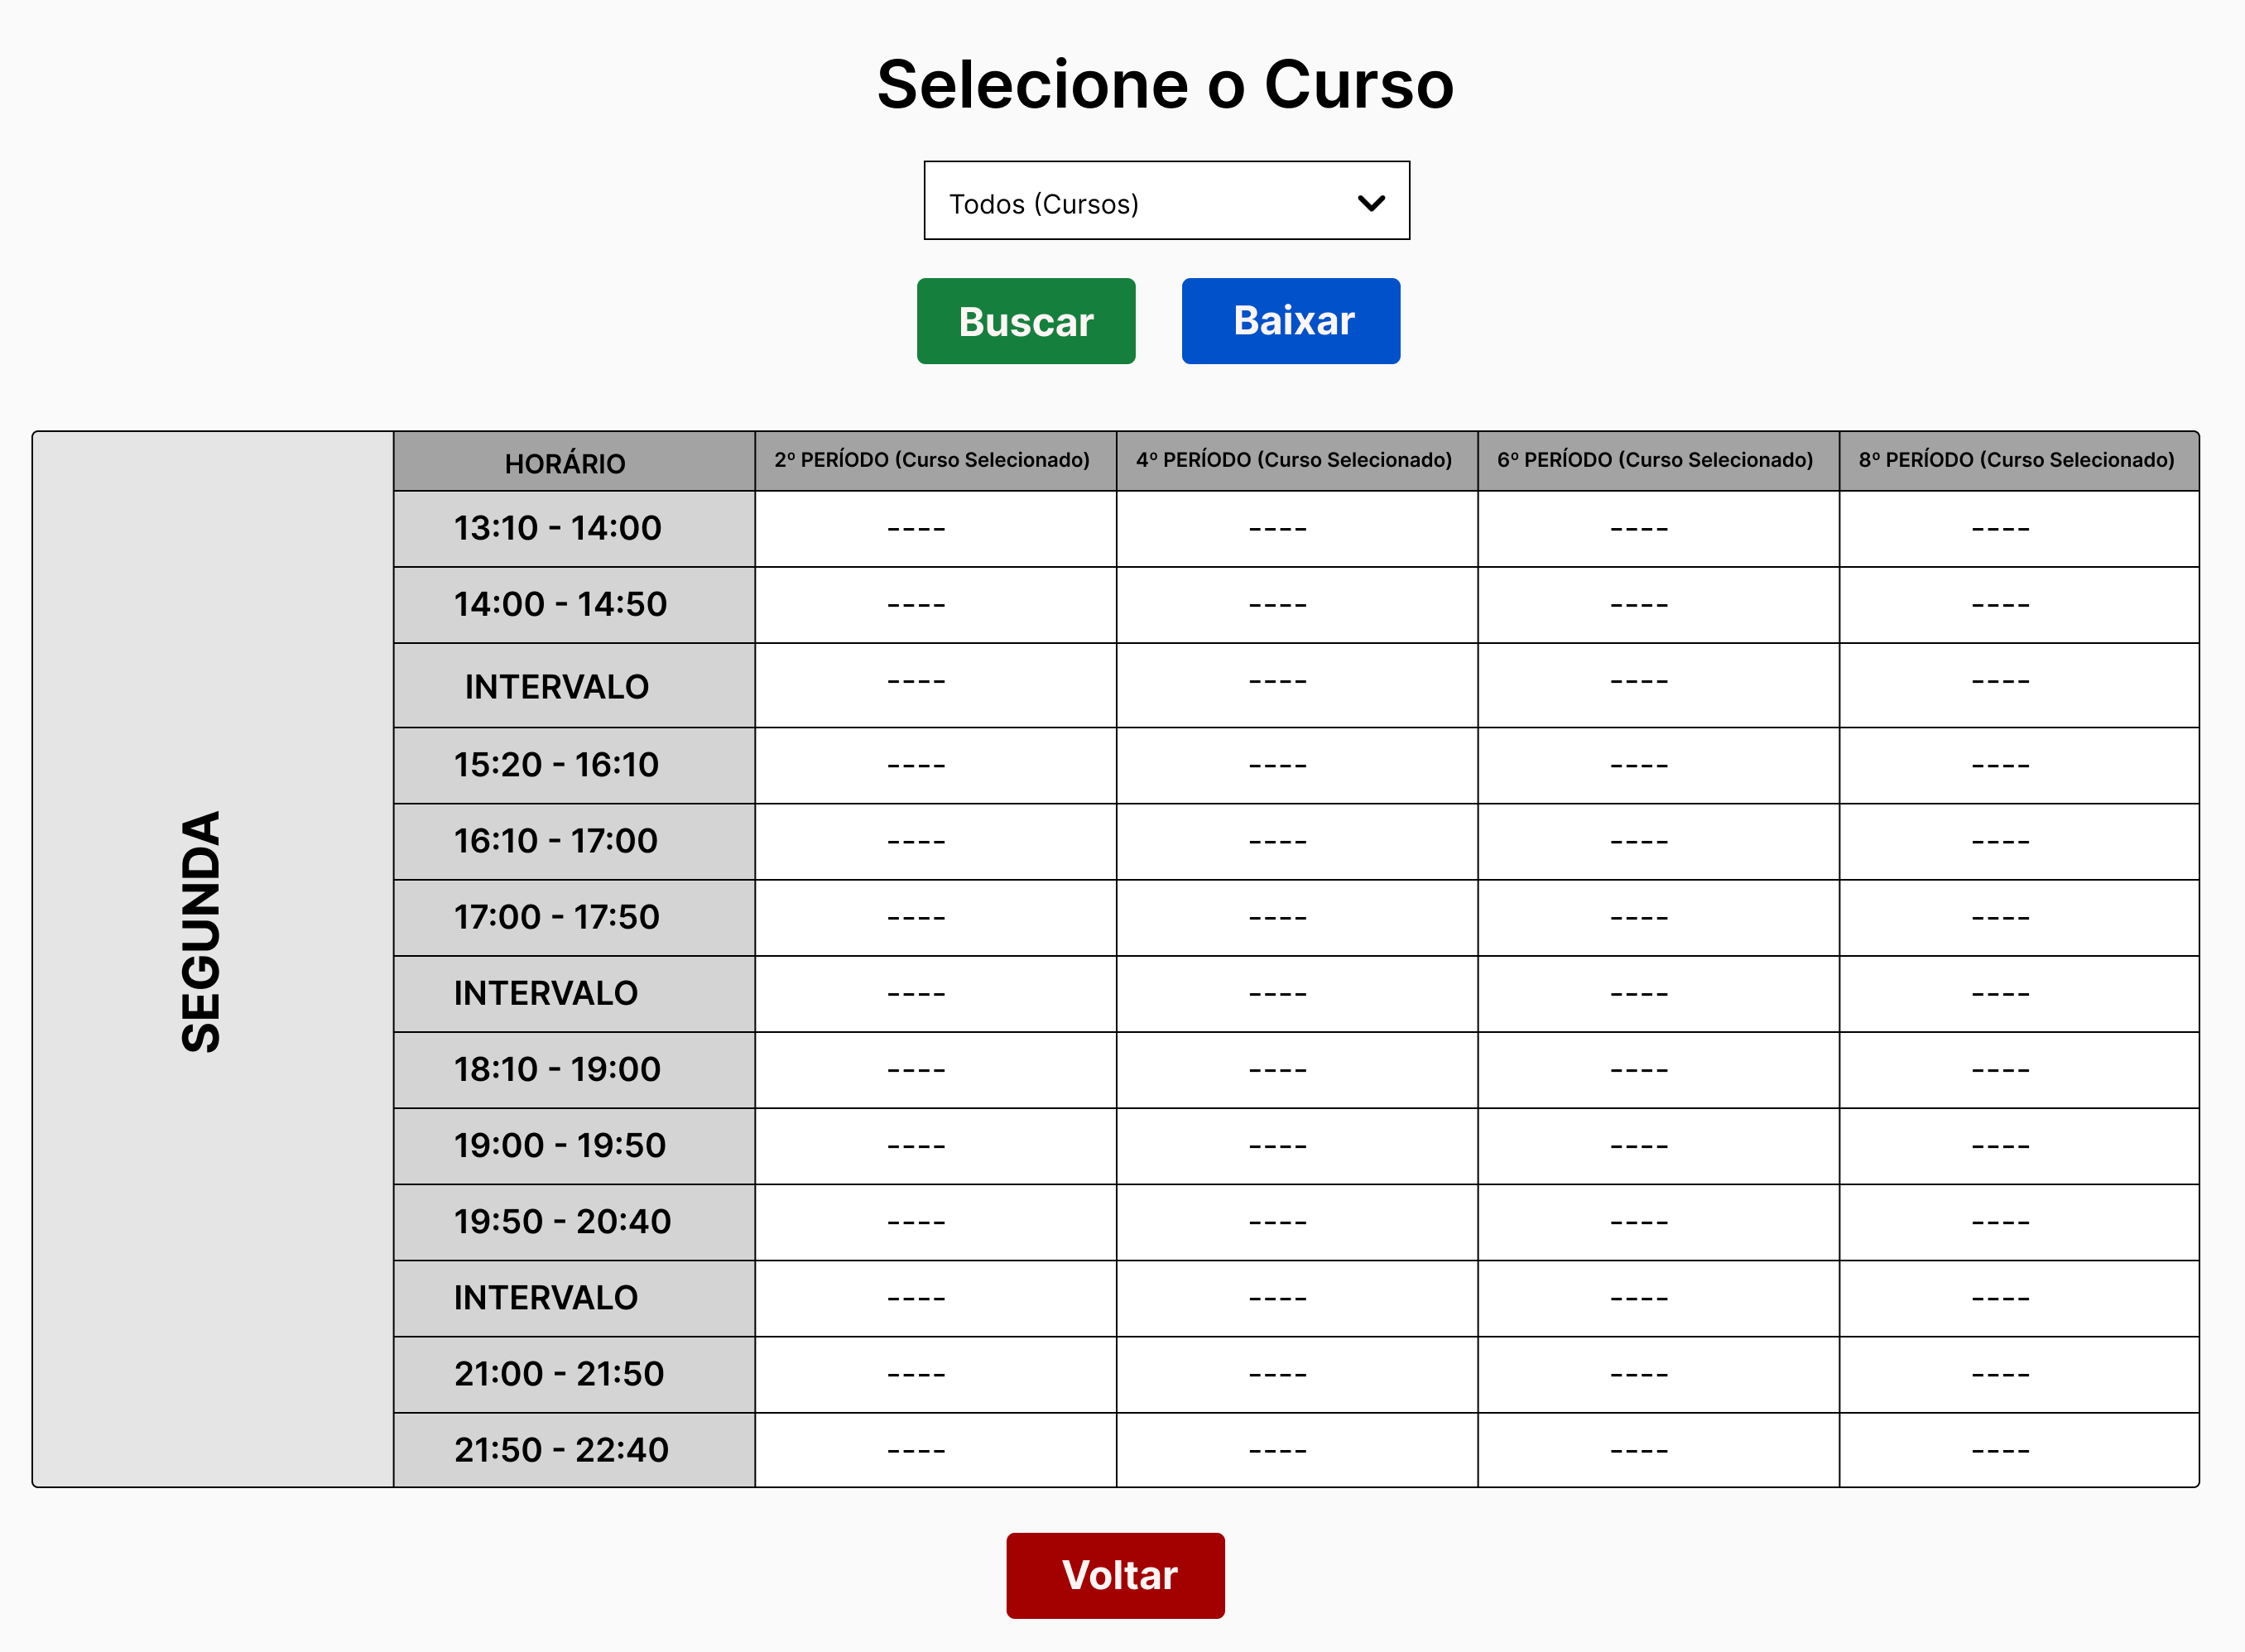
\includegraphics[width=1\textwidth]{Figuras/proto-3.PNG}
    \caption*{Fonte: AUTOR (2024)}
    \label{fig_proto_3}
\end{figure}

As Figuras \ref{fig_proto_2} e \ref{fig_proto_3} apresentam o protótipo da tela dos cursos, exibindo os horários e a distribuição das aulas ao longo da semana para um curso selecionado.

\begin{figure}[htb]
    \centering
    \caption{Protótipo da tela dos professores}
    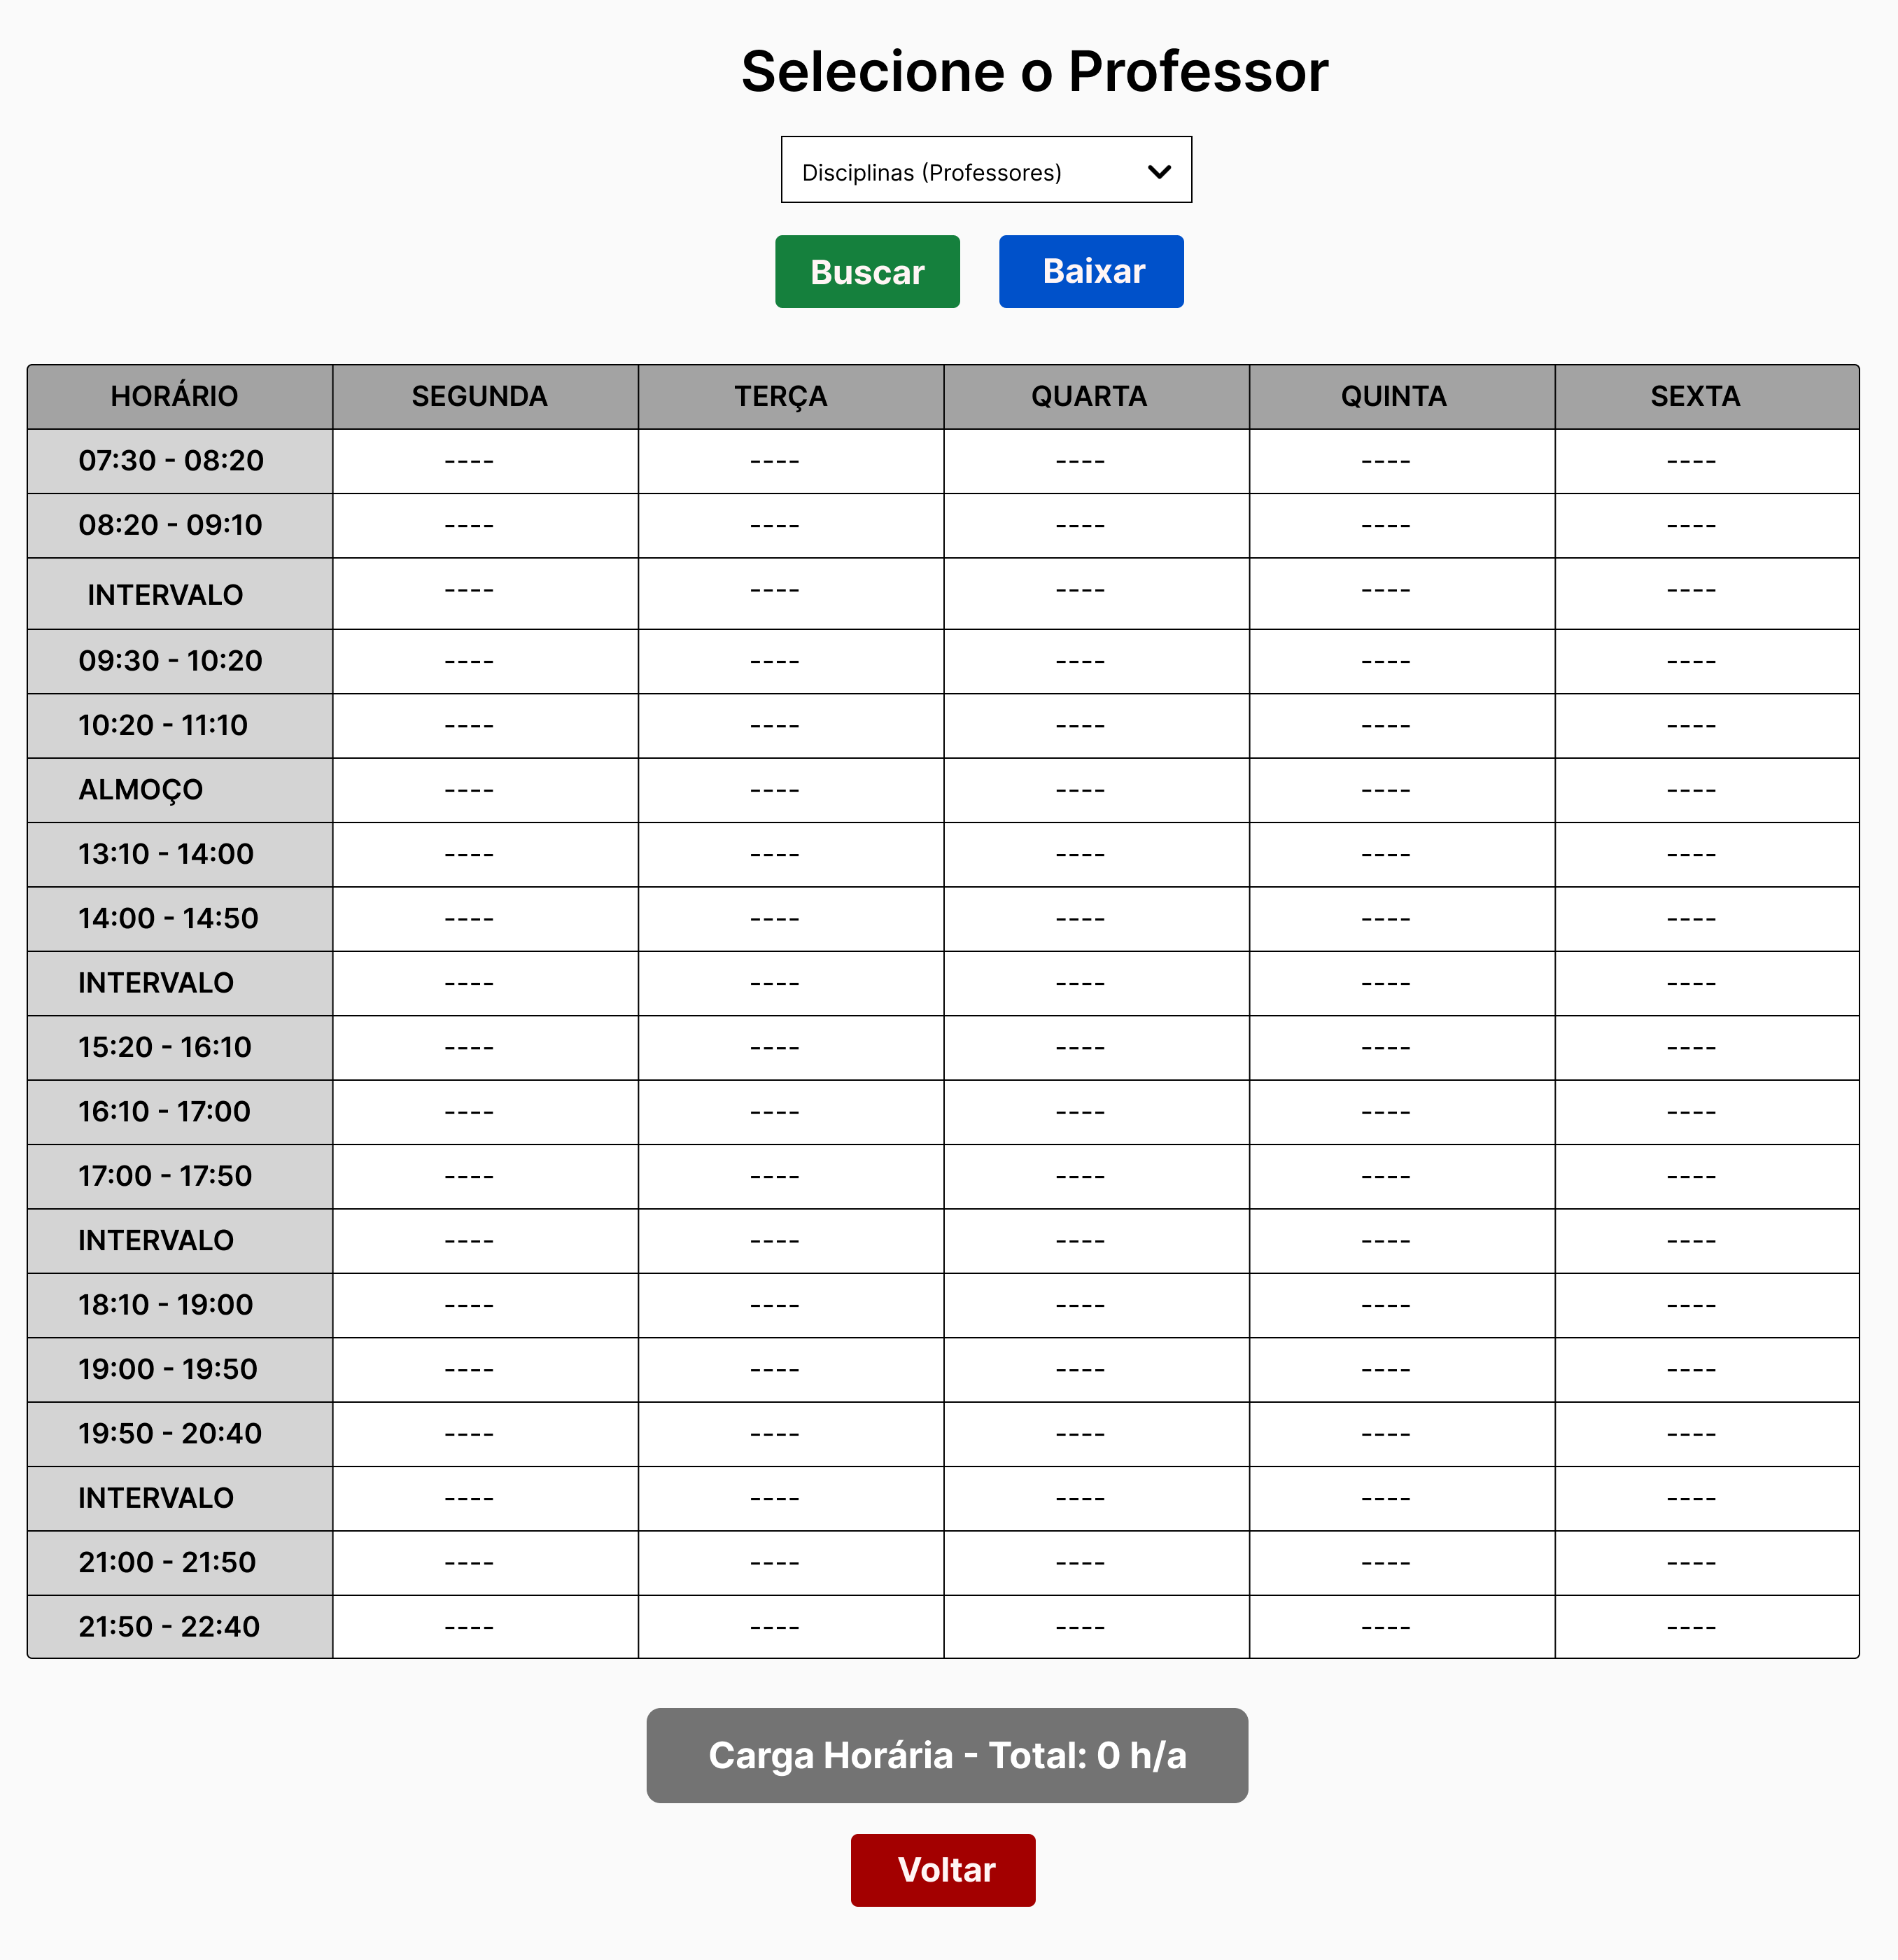
\includegraphics[width=1\textwidth]{Figuras/proto-4.PNG}
    \caption*{Fonte: AUTOR (2024)}
    \label{fig_proto_4}
\end{figure}

A Figura \ref{fig_proto_4} mostra o protótipo da tela dos professores, detalhando os horários das aulas e os dias da semana de um professor escolhido.

\begin{figure}[H]
    \centering
    \caption{Protótipo da tela das salas}
    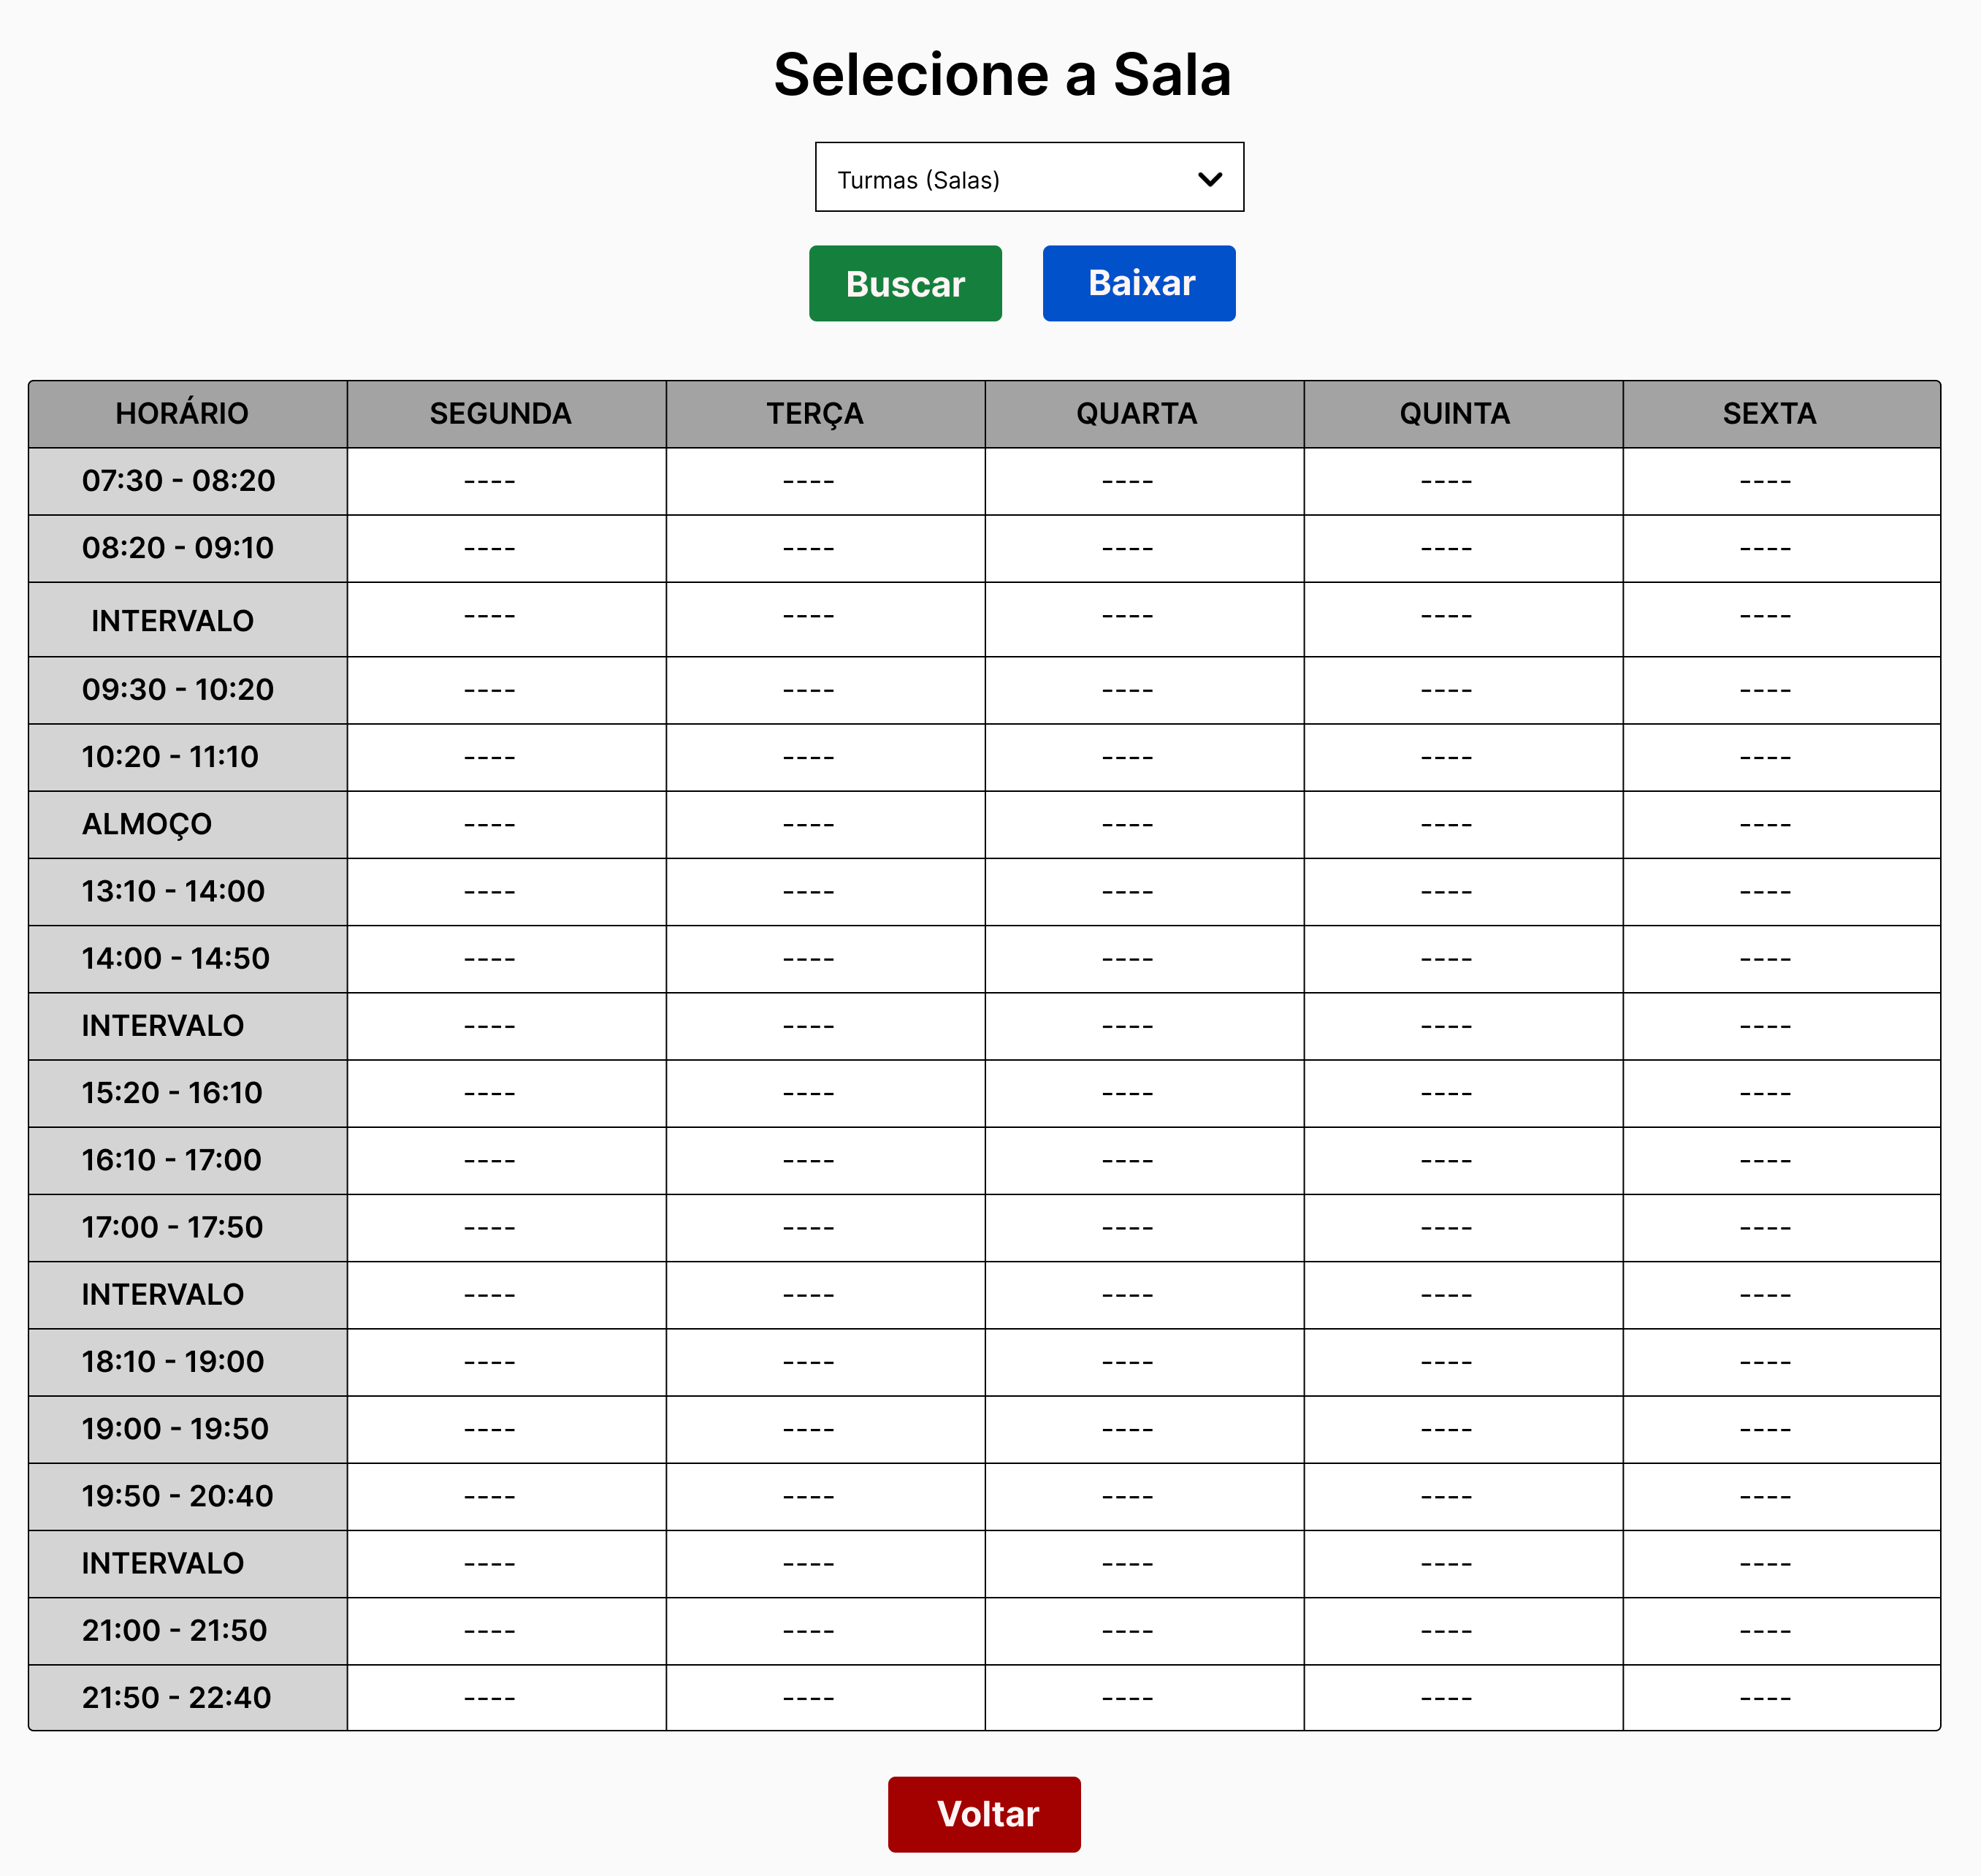
\includegraphics[width=1\textwidth]{Figuras/proto-5.PNG}
    \caption*{Fonte: AUTOR (2024)}
    \label{fig_proto_5}
\end{figure}

A Figura \ref{fig_proto_5} apresenta o protótipo da tela das salas, exibindo os horários de ocupação e os dias em que uma sala está reservada.

\subsection{Desenvolvimento do Front-end}

O front-end foi desenvolvido com o Next.js. Essa tecnologia possibilitou criar uma interface moderna e eficiente, capaz de responder dinamicamente a eventos e mudanças de estado, garantindo uma experiência de usuário fluida e responsiva. Todo o trabalho priorizou clareza na organização dos componentes, reutilização de elementos e facilidade de futuras evoluções, atendendo às necessidades do projeto com agilidade. O código está disponível no repositório do projeto em \url{https://github.com/Tomaz5556/Horarios-IFNMG-Salinas}. A seguir, são exibidas as telas resultantes desse processo:

\begin{figure}[htb]
    \centering
    \caption{Menu principal com opções de botões de horários e outros serviços}
    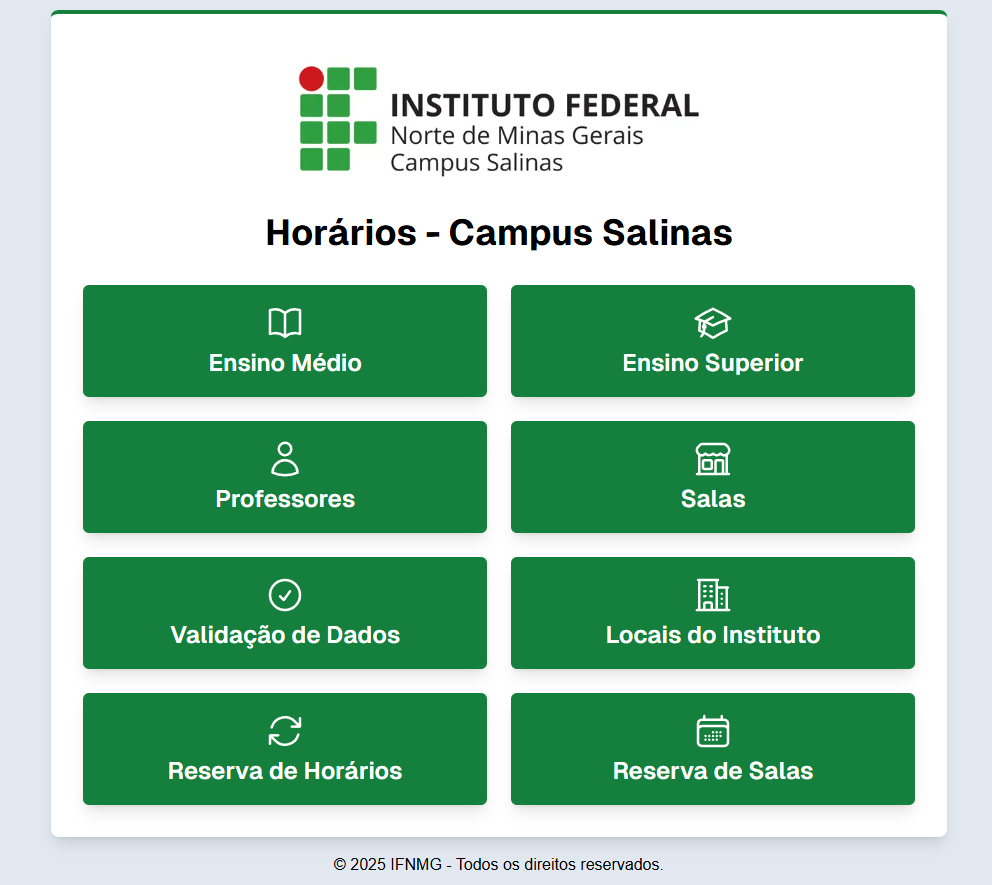
\includegraphics[width=1\textwidth]{Figuras/front-1.png}
    \caption*{Fonte: AUTOR (2025)}
    \label{fig_front_1}
\end{figure}

A Figura \ref{fig_front_1} mostra o menu principal da plataforma, com botões para consulta de horários e acesso a outros serviços.

\begin{figure}[htb]
    \centering
    \caption{Tela dos cursos}
    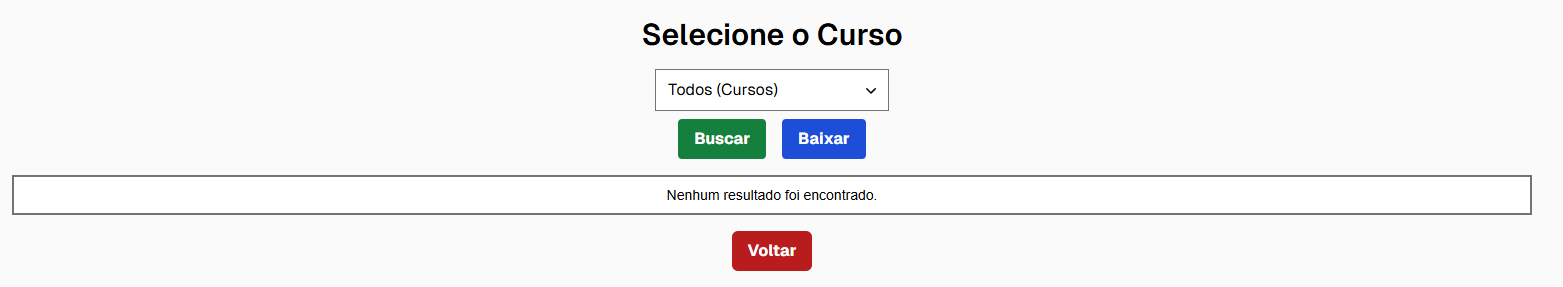
\includegraphics[width=1\textwidth]{Figuras/front-2.png}
    \caption*{Fonte: AUTOR (2025)}
    \label{fig_front_2}
\end{figure}

A Figura \ref{fig_front_2} apresenta a tela dos cursos, permitindo selecionar turmas e visualizar seus horários.

\begin{figure}[htb]
    \centering
    \caption{Tela dos cursos com cursos técnicos}
    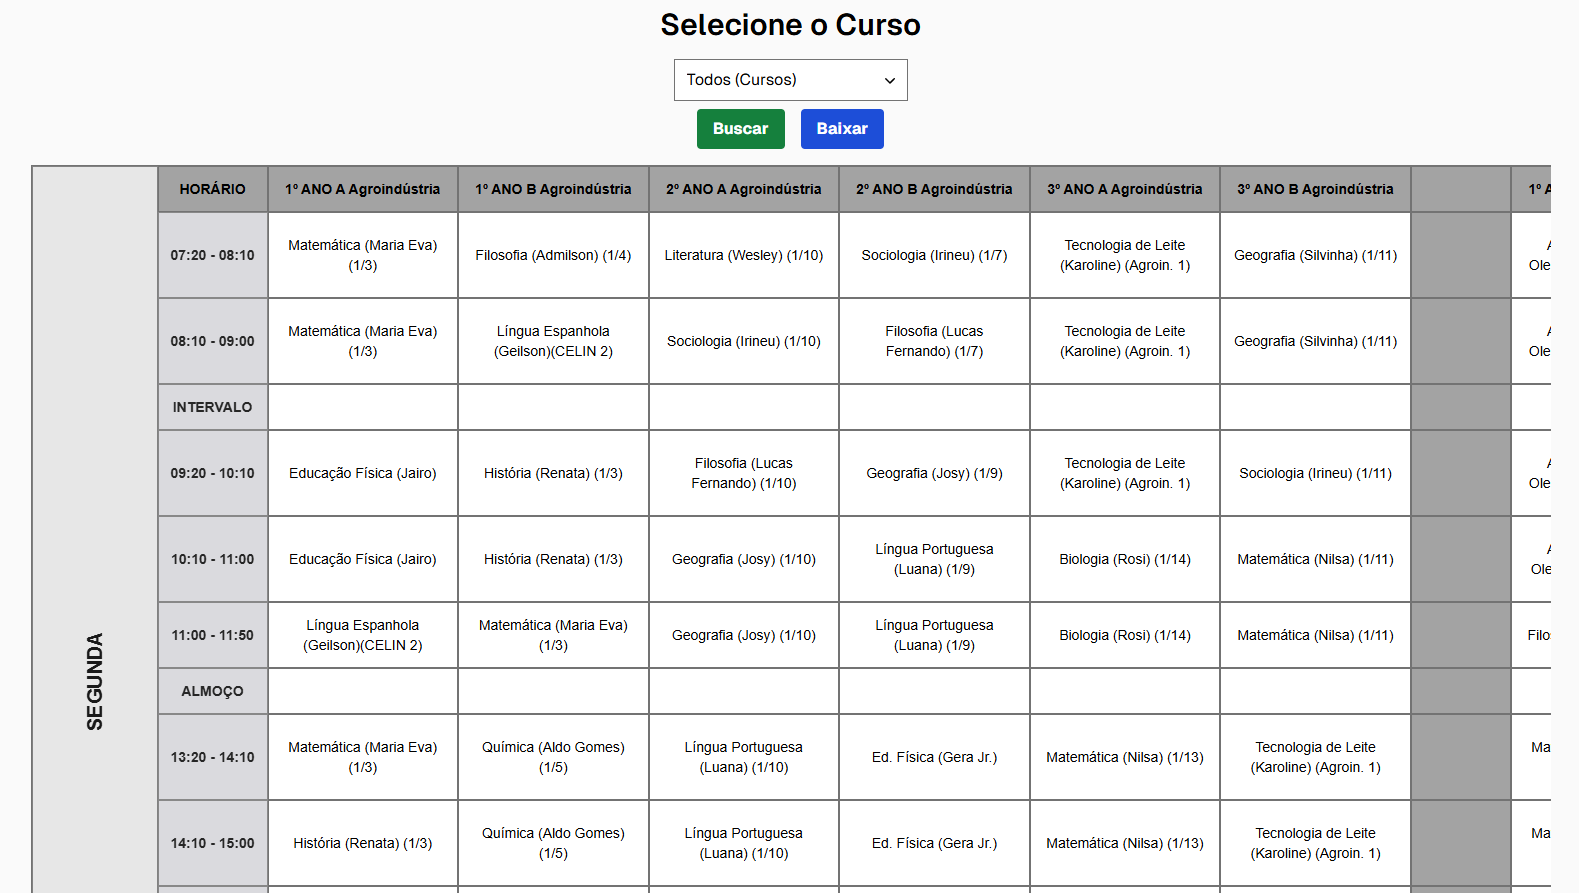
\includegraphics[width=1\textwidth]{Figuras/front-3.png}
    \caption*{Fonte: AUTOR (2025)}
    \label{fig_front_3}
\end{figure}

\begin{figure}[H]
    \centering
    \caption{Tela dos cursos com cursos superiores}
    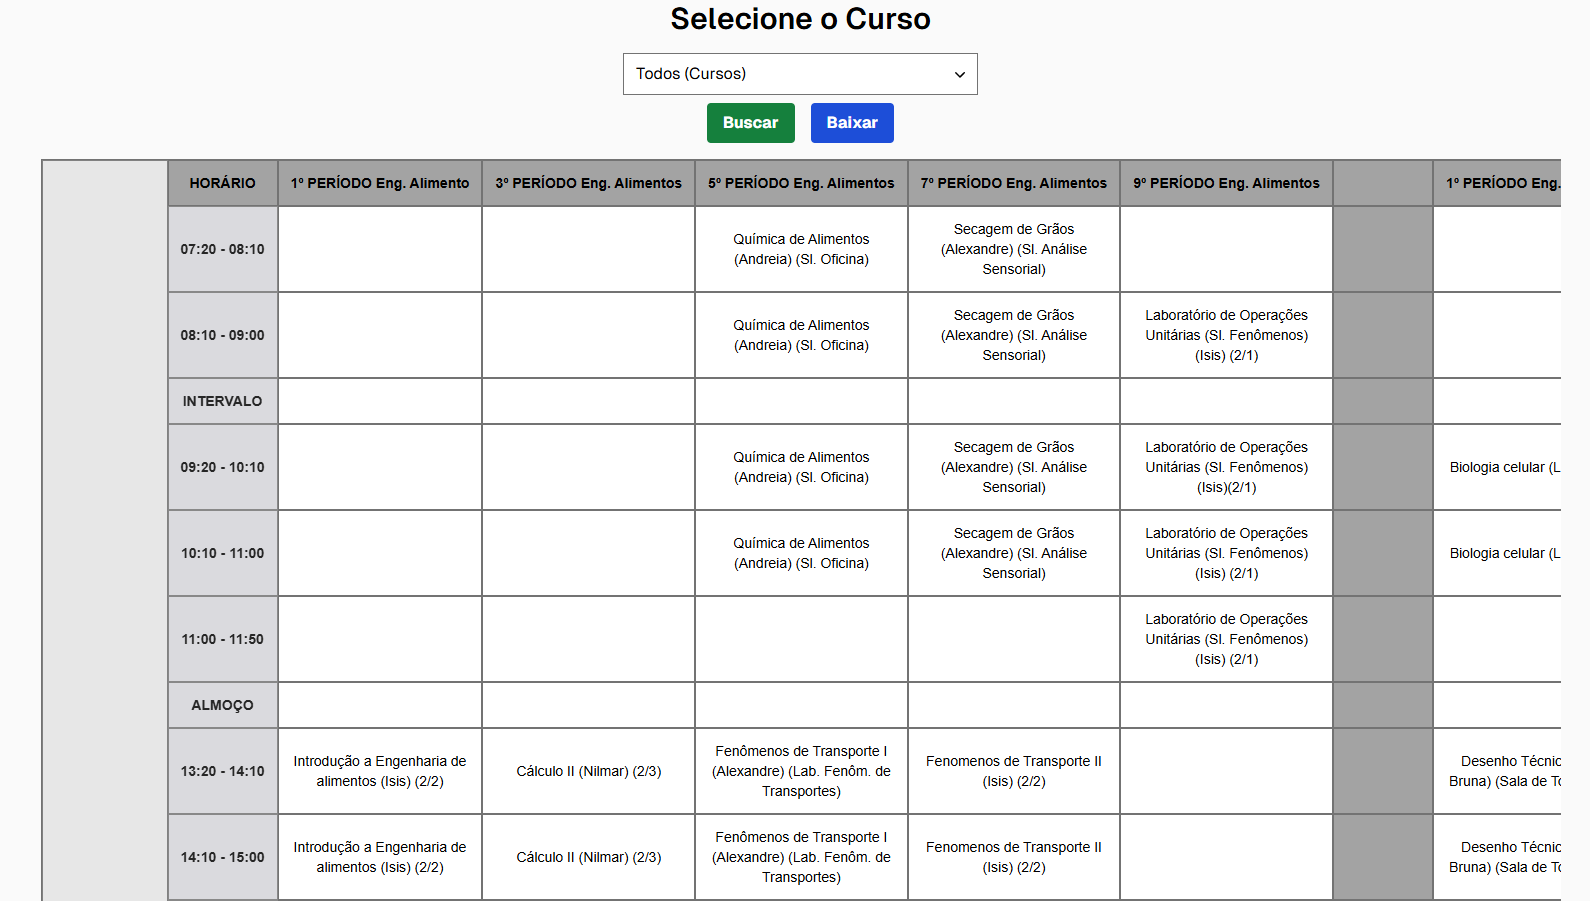
\includegraphics[width=1\textwidth]{Figuras/front-4.png}
    \caption*{Fonte: AUTOR (2025)}
    \label{fig_front_4}
\end{figure}

As Figuras \ref{fig_front_3} e \ref{fig_front_4} detalham, respectivamente, a exibição dos horários para cursos técnicos e superiores.

\begin{figure}[htb]
    \centering
    \caption{Tela dos professores}
    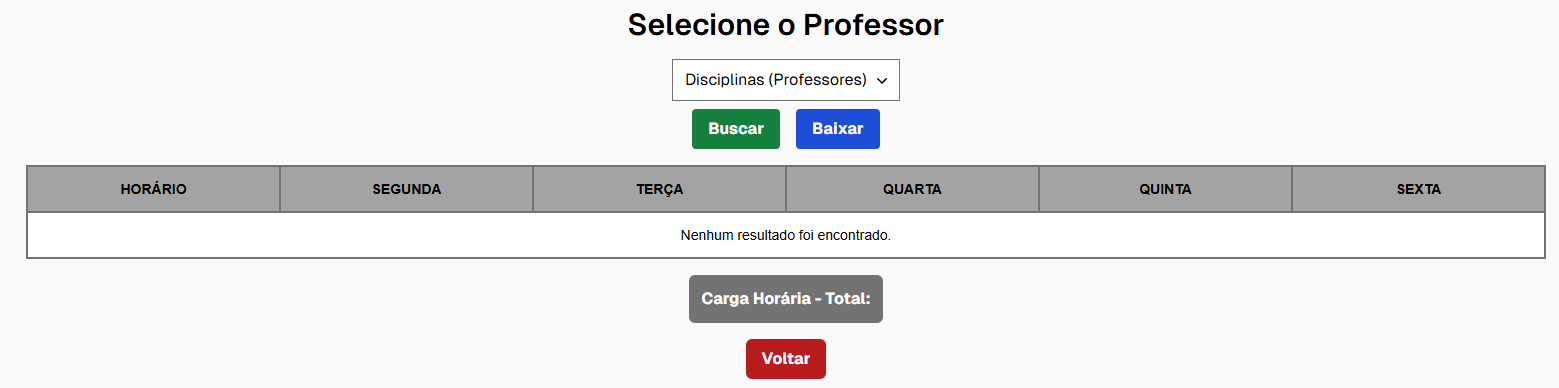
\includegraphics[width=1\textwidth]{Figuras/front-5.png}
    \caption*{Fonte: AUTOR (2025)}
    \label{fig_front_5}
\end{figure}

\begin{figure}[H]
    \centering
    \caption{Tela dos professores com um professor selecionado}
    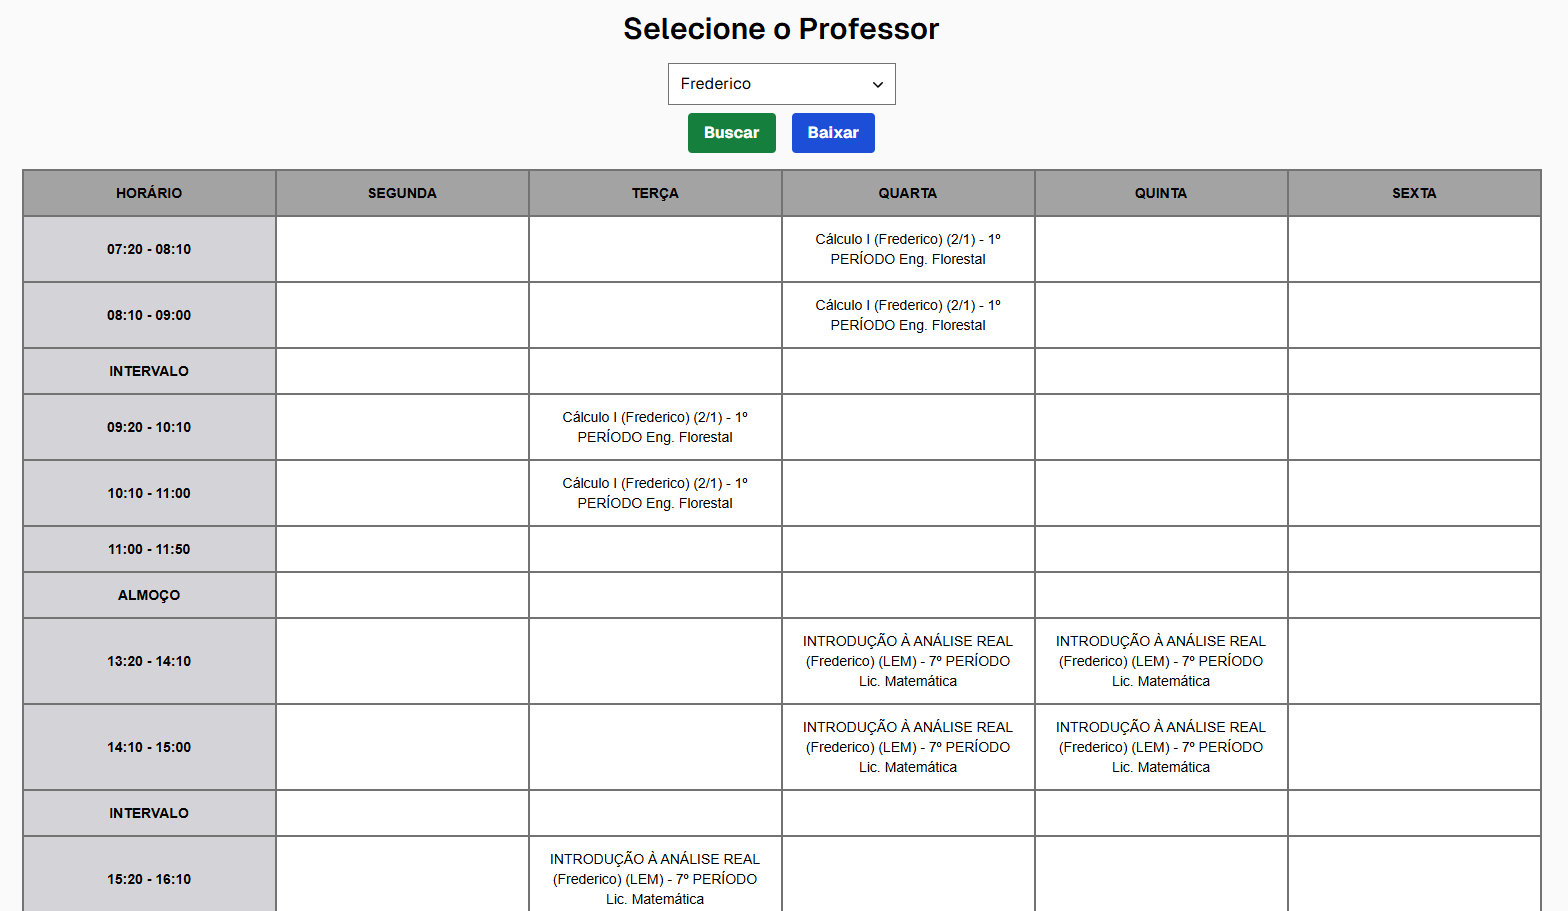
\includegraphics[width=1\textwidth]{Figuras/front-6.png}
    \caption*{Fonte: AUTOR (2025)}
    \label{fig_front_6}
\end{figure}

A Figura \ref{fig_front_5} ilustra a tela dos professores, enquanto a Figura \ref{fig_front_6} exibe um professor selecionado, com seus horários organizados.

\begin{figure}[H]
    \centering
    \caption{Tela das salas}
    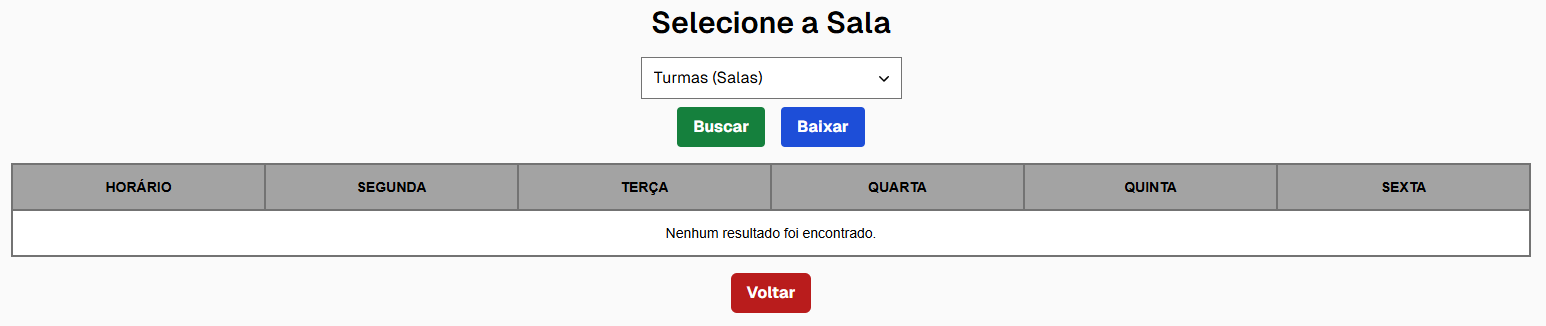
\includegraphics[width=1\textwidth]{Figuras/front-7.png}
    \caption*{Fonte: AUTOR (2025)}
    \label{fig_front_7}
\end{figure}

\begin{figure}[htb]
    \centering
    \caption{Tela das salas com uma sala selecionada}
    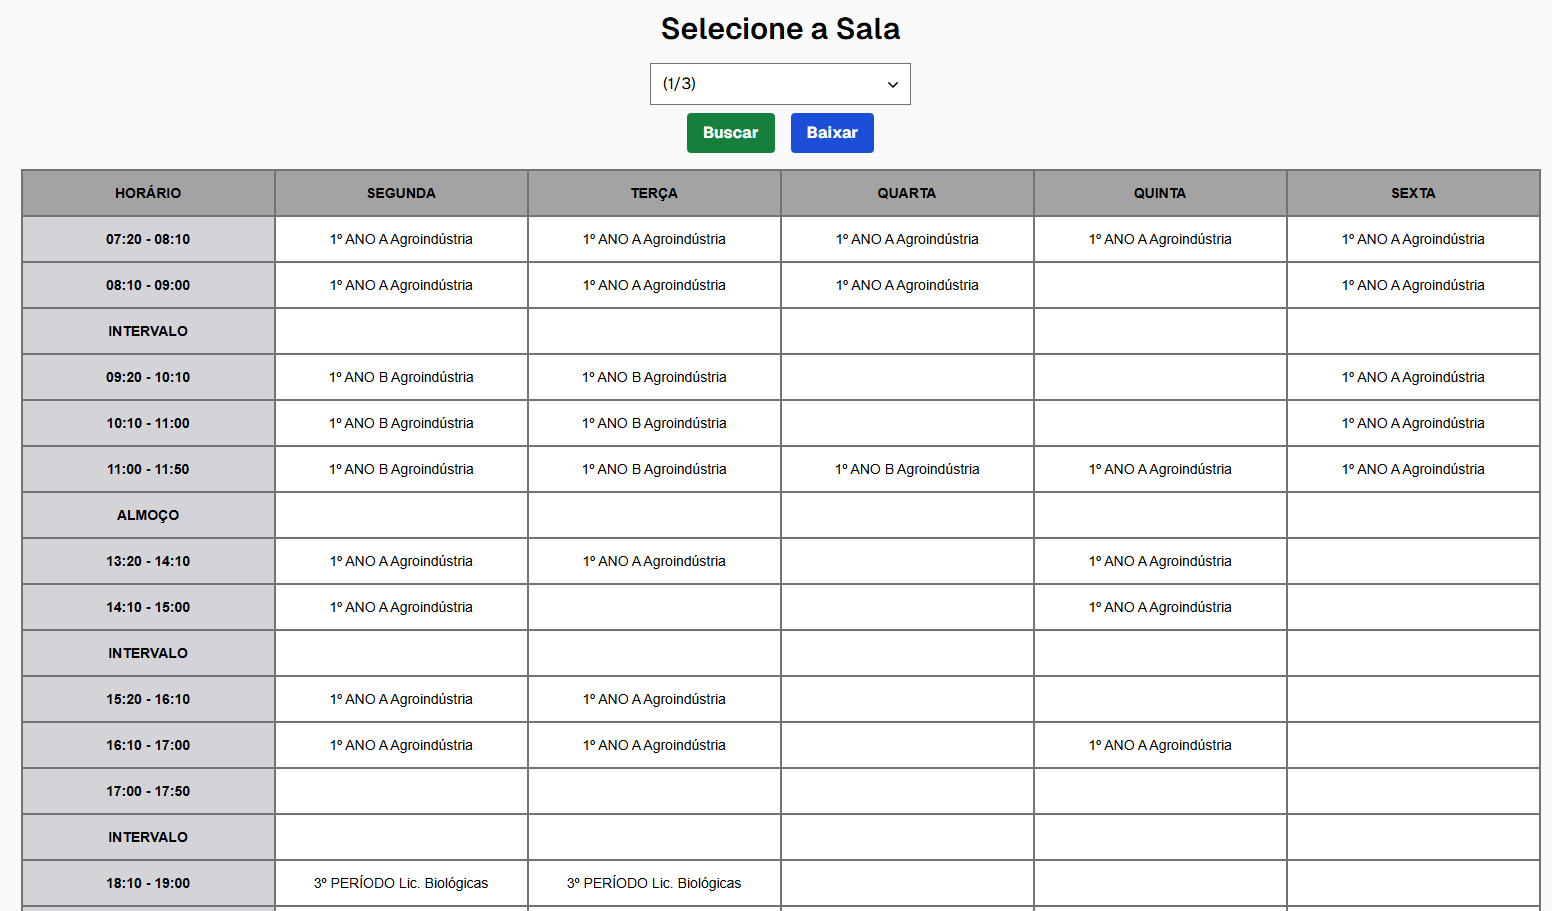
\includegraphics[width=1\textwidth]{Figuras/front-8.png}
    \caption*{Fonte: AUTOR (2025)}
    \label{fig_front_8}
\end{figure}

A Figura \ref{fig_front_7} apresenta a tela das salas e a Figura \ref{fig_front_8} mostra a visualização de uma sala específica com seu cronograma de uso.

\begin{figure}[htb]
    \centering
    \caption{Tela de login para acessar a tela de validação}
    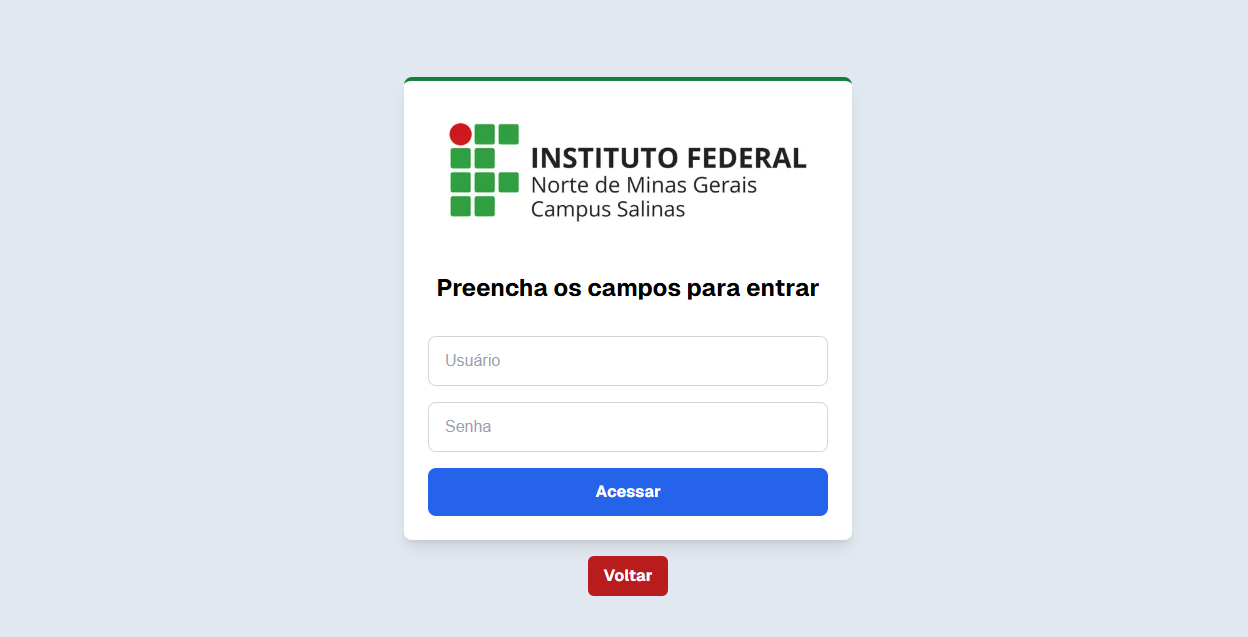
\includegraphics[width=1\textwidth]{Figuras/front-9.png}
    \caption*{Fonte: AUTOR (2025)}
    \label{fig_front_9}
\end{figure}

\begin{figure}[H]
    \centering
    \caption{Tela de validação}
    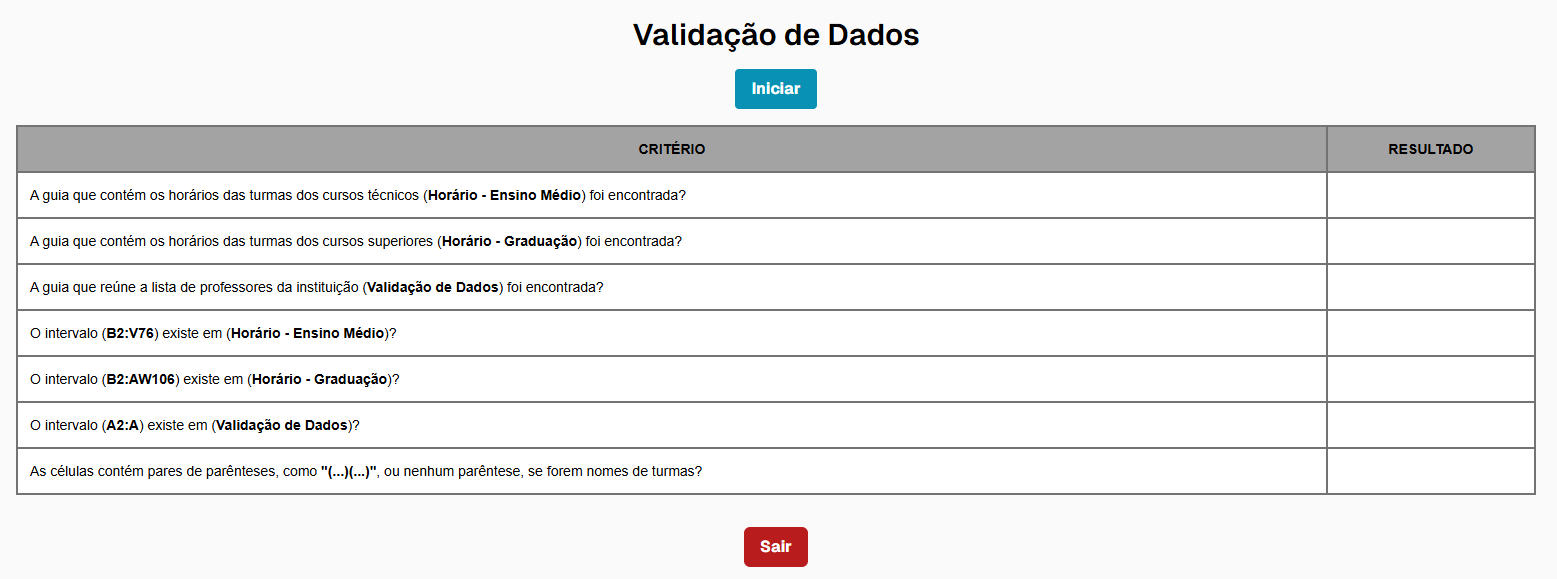
\includegraphics[width=1\textwidth]{Figuras/front-10.png}
    \caption*{Fonte: AUTOR (2025)}
    \label{fig_front_10}
\end{figure}

Já a Figura \ref{fig_front_9} traz a tela de login para acessar a área de validação de dados, e a Figura \ref{fig_front_10} mostra a tela de validação.

\begin{figure}[htb]
    \centering
    \caption{Sistema que exibe os locais do instituto}
    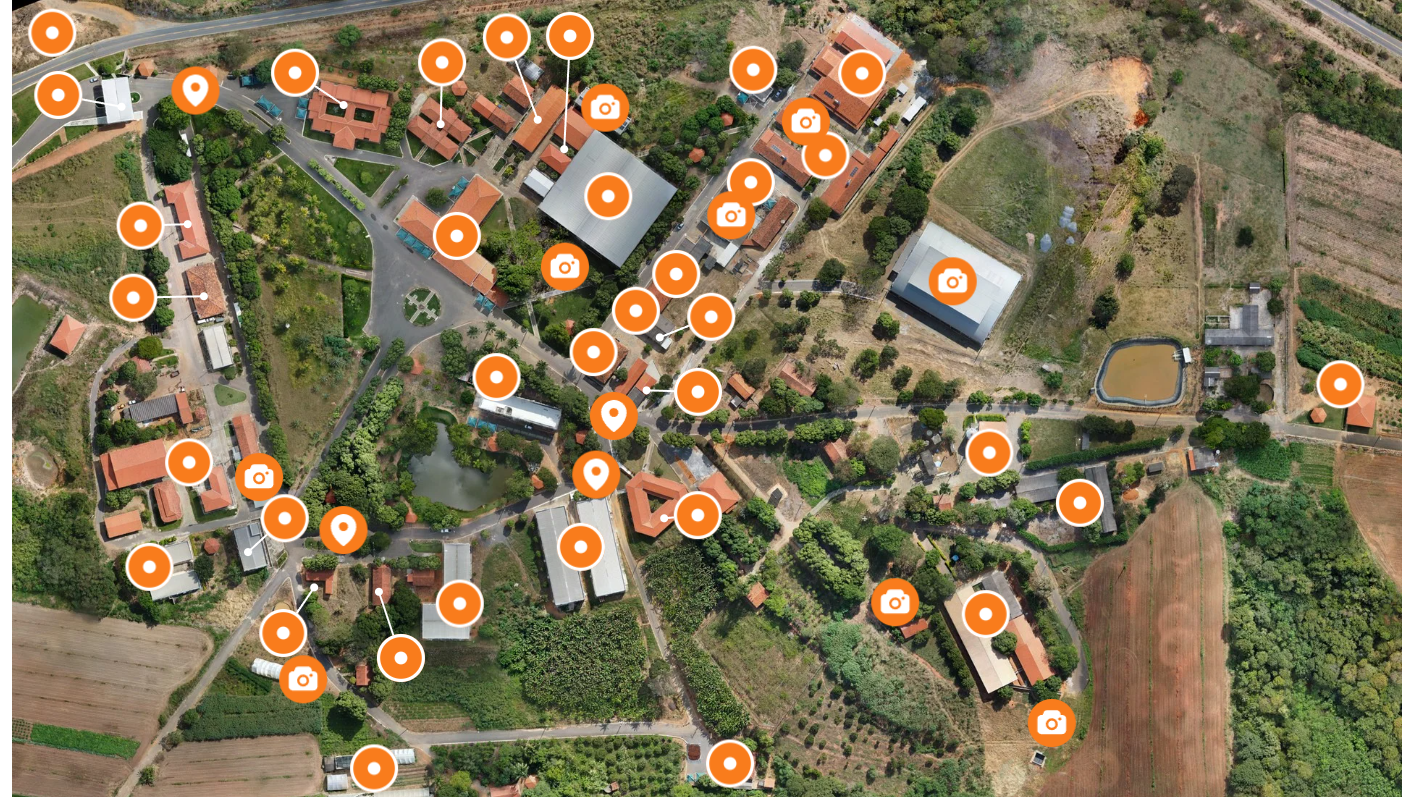
\includegraphics[width=1\textwidth]{Figuras/front-11.png}
    \caption*{Fonte: AUTOR (2025)}
    \label{fig_front_11}
\end{figure}

\begin{figure}[H]
    \centering
    \caption{Sistema de reserva de horários}
    
\includegraphics[width=1\textwidth]{Figuras/front-12.png}
    \caption*{Fonte: AUTOR (2025)}
    \label{fig_front_12}
\end{figure}

\begin{figure}[htb]
    \centering
    \caption{Sistema de gerenciamento de reserva de salas}
    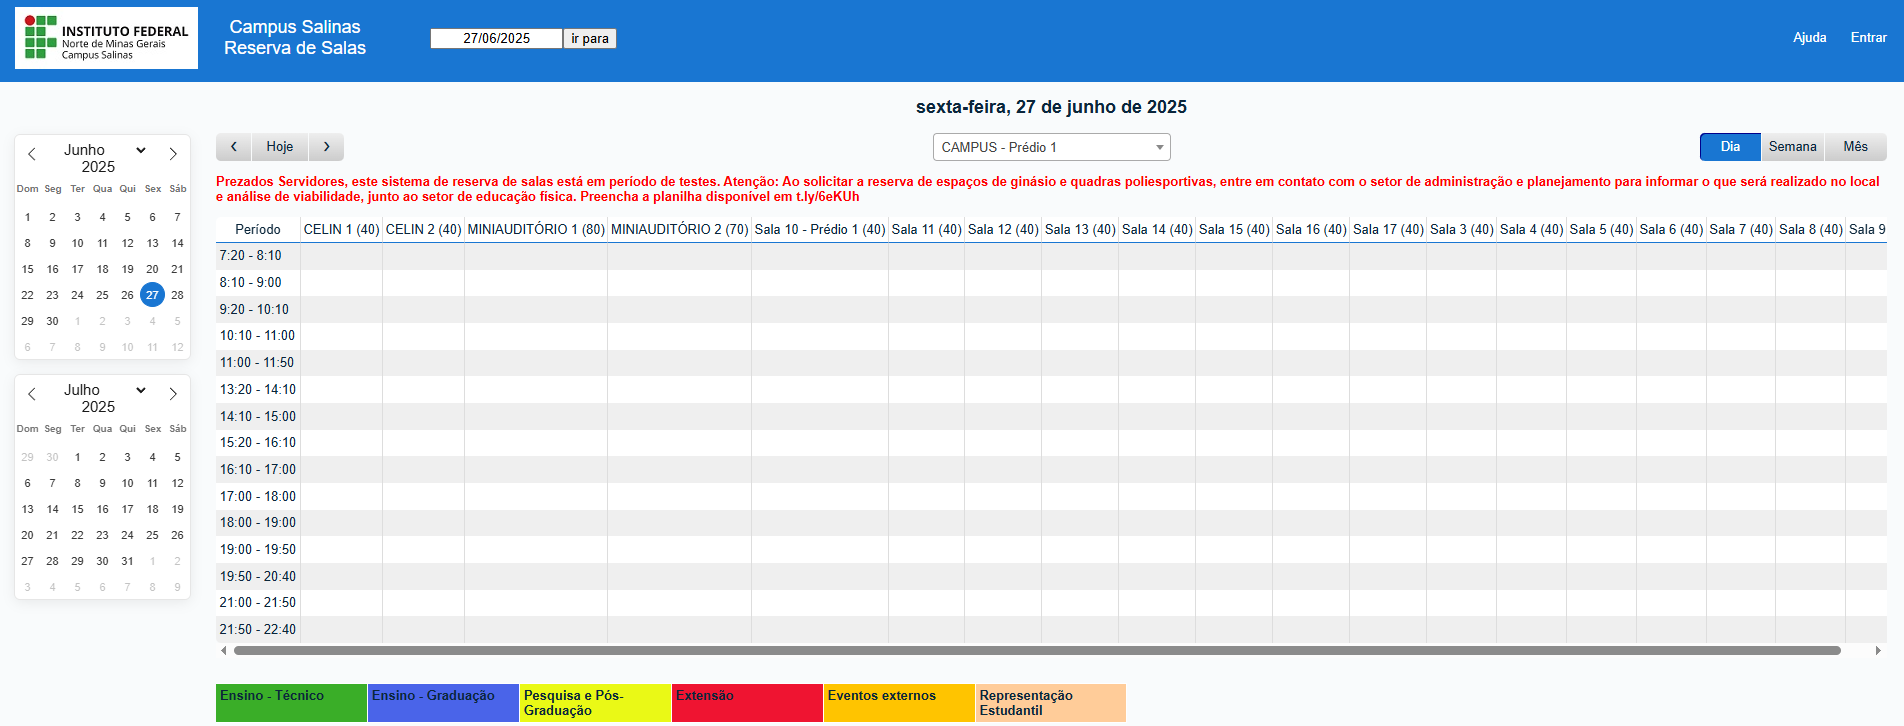
\includegraphics[width=1\textwidth]{Figuras/front-13.png}
    \caption*{Fonte: AUTOR (2025)}
    \label{fig_front_13}
\end{figure}

Por fim, as Figuras \ref{fig_front_11}, \ref{fig_front_12} e \ref{fig_front_13} ilustram os sistemas externos integrados à plataforma, incluindo a visualização de locais do instituto, o sistema de reserva de horários e o gerenciamento de reservas de salas. Esses sistemas, embora estejam acessíveis a partir da plataforma desenvolvida, não fazem parte do escopo desse trabalho.

\subsection{Estrutura do Front-end}

A estrutura do front-end está organizada de forma modular, visando clareza, manutenção facilitada e reutilização de código. Na Figura \ref{fig_front_14}, destacam-se os principais elementos:

\begin{figure}[htb]
    \centering
    \caption{Estrutura do front-end}
    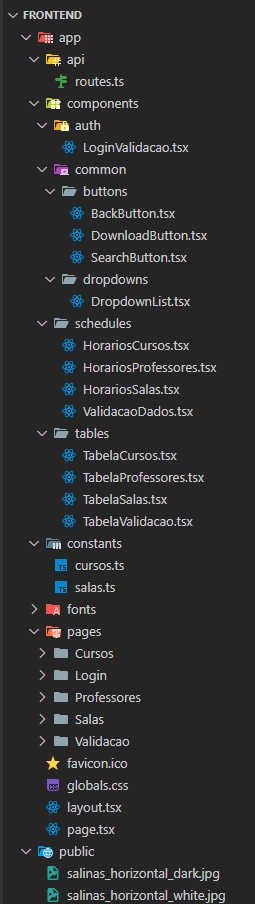
\includegraphics[width=0.25\textwidth]{Figuras/front-14.png}
    \caption*{Fonte: AUTOR (2025)}
    \label{fig_front_14}
\end{figure}

\begin{itemize}
    \item api: pasta responsável por buscar dados da planilha por meio de requisições, contando com o arquivo routes.ts para gerenciar essas chamadas.
    \item components: pasta que centraliza os componentes do sistema, subdividida em:
    \begin{itemize}
        \item auth: pasta responsável pelo controle de autenticação, incluindo o arquivo LoginValidacao.tsx, que verifica as credenciais de login antes de entrar na tela de validação.
        \item common: pasta destinada a componentes reutilizáveis, contendo:
        \begin{itemize}
            \item buttons: reúne botões de ação como BackButton.tsx (retorno), DownloadButton.tsx (download de tabelas) e SearchButton.tsx (busca de horários).
             \item dropdowns: responsável pelas listas suspensas, como o arquivo DropdownList.tsx, utilizado para seleção de cursos, professores ou salas.
        \end{itemize}
        \item schedules: pasta com componentes independentes para exibição de horários, como HorariosCursos.tsx, HorariosProfessores.tsx, HorariosSalas.tsx e ValidacaoDados.tsx.
        \item tables: pasta com componentes independentes para apresentação das tabelas com os dados, incluindo TabelaCursos.tsx, TabelaProfessores.tsx, TabelaSalas.tsx e TabelaValidacao.tsx.
    \end{itemize}
    \item constants: pasta responsável por definir as listas de cursos e salas disponíveis, armazenadas nos arquivos cursos.ts e salas.ts.
    \item pages: organiza as rotas da aplicação, com páginas específicas para cursos, professores, salas, login e validação.
    \item globals.css: arquivo de estilos globais aplicados em toda a interface.
    \item layout.tsx: define a estrutura geral de layout e permite a edição de metadados de forma centralizada.
    \item page.tsx: página inicial que exibe o menu principal com opções de botões de horários e outros serviços.
    \item public: pasta com imagens do logotipo institucional do IFNMG Campus Salinas, disponibilizadas tanto na versão padrão quanto na versão em preto e branco.
\end{itemize}

\subsection{Funcionalidades do Front-end}

\begin{itemize}
    \item Modo escuro: adapta automaticamente o tema da aplicação (claro ou escuro) de acordo com a configuração do navegador, oferecendo maior conforto visual aos usuários. A seguir, será mostrado na Figura \ref{fig_front_15}.

    \begin{figure}[H]
        \centering
        \caption{Modo escuro}
        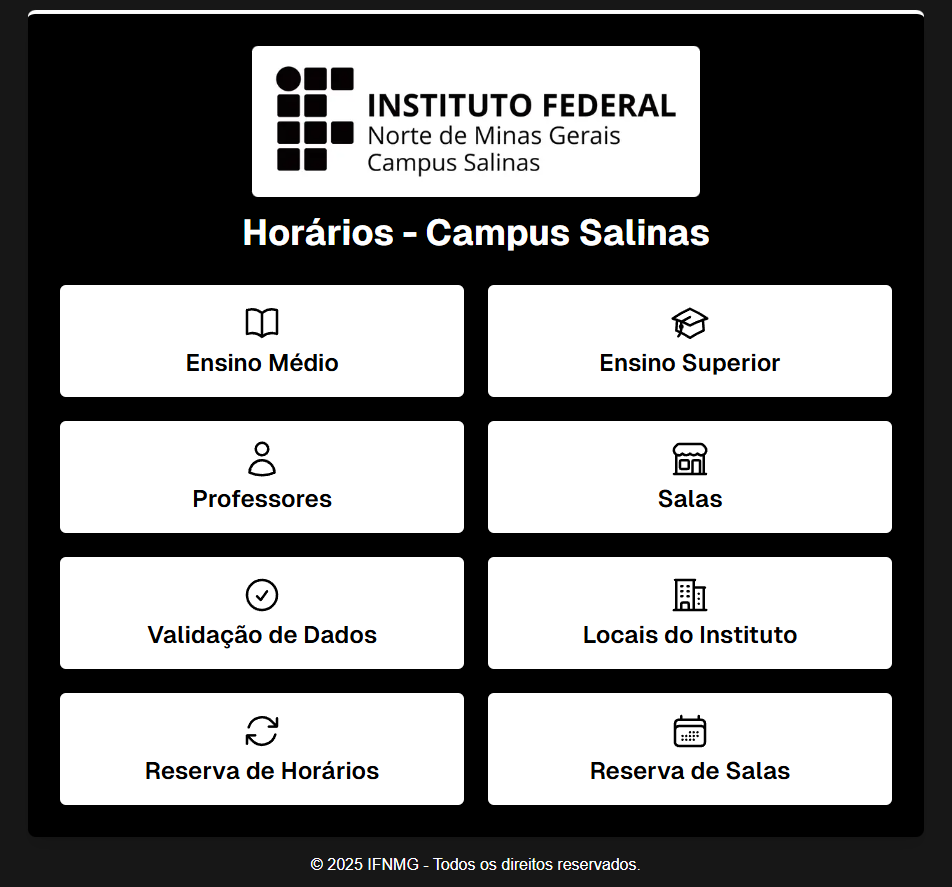
\includegraphics[width=0.9\textwidth]{Figuras/front-15.png}
        \caption*{Fonte: AUTOR (2025)}
        \label{fig_front_15}
    \end{figure}

    \item Responsividade: garante que a interface funcione bem tanto em dispositivos móveis quanto em desktops, mantendo a usabilidade e a organização dos elementos. Ver Figura \ref{fig_front_16}.

    \begin{figure}[H]
        \centering
        \caption{Responsividade}
        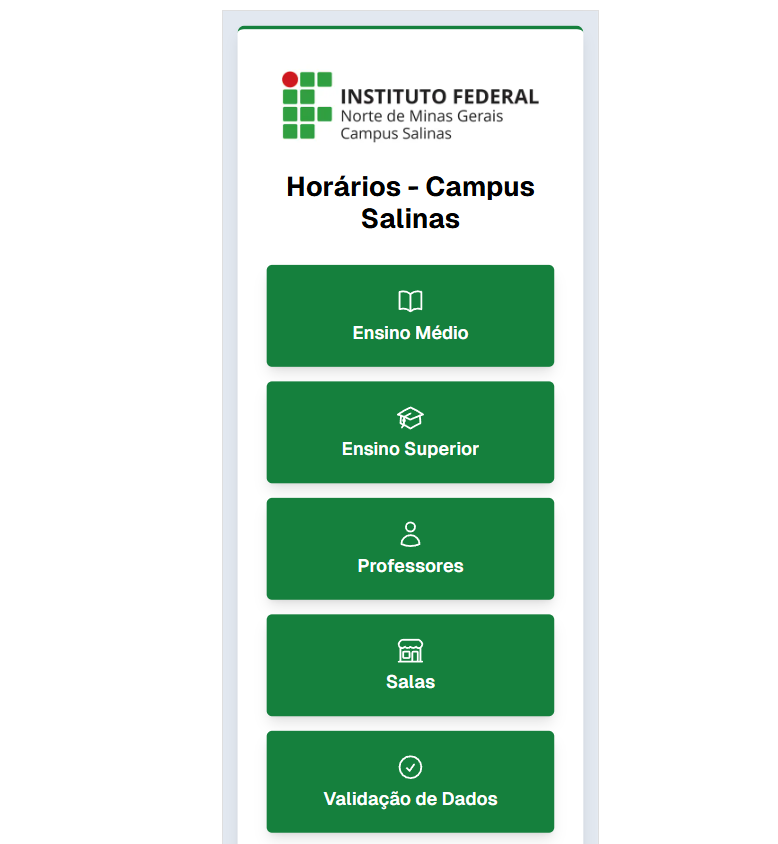
\includegraphics[width=0.3\textwidth]{Figuras/front-16.png}
        \caption*{Fonte: AUTOR (2025)}
        \label{fig_front_16}
    \end{figure}
    
    \item Busca de horários de cursos: possibilita consultar os horários dos cursos técnicos e superiores, exibindo os dias e horários de segunda a sexta-feira. Apresentado na Figura \ref{fig_front_17}.

    \begin{figure}[htb]
        \centering
        \caption{Busca de horários de cursos}
        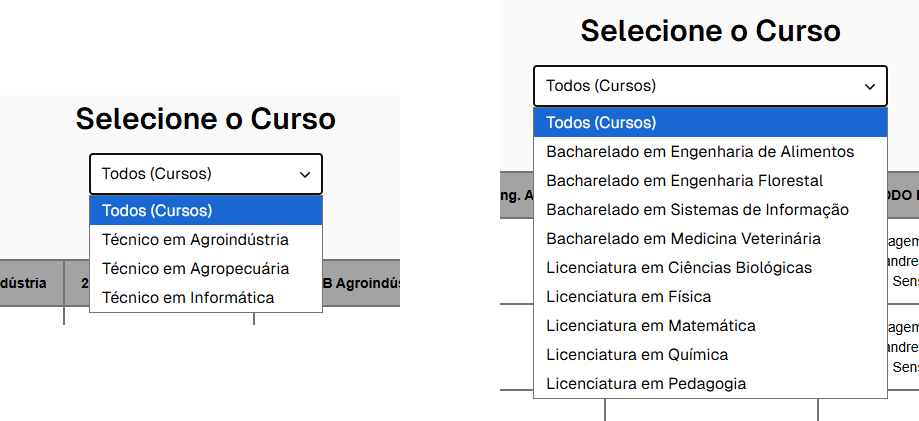
\includegraphics[width=0.6\textwidth]{Figuras/front-17.png}
        \caption*{Fonte: AUTOR (2025)}
        \label{fig_front_17}
    \end{figure}
    
    \item Busca de horários de professores: permite selecionar um professor em uma lista suspensa e visualizar seus horários semanais completos. Ilustrado na Figura \ref{fig_front_18}.

    \begin{figure}[H]
        \centering
        \caption{Busca de horários de professores}
        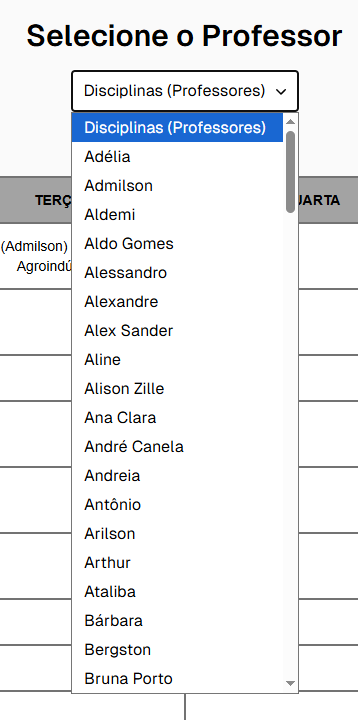
\includegraphics[width=0.2\textwidth]{Figuras/front-18.png}
        \caption*{Fonte: AUTOR (2025)}
        \label{fig_front_18}
    \end{figure}
    
    \item Busca de horários de salas: possibilita selecionar uma sala em uma lista suspensa e consultar os horários de ocupação de segunda a sexta-feira. Mostrado na Figura \ref{fig_front_19}.

    \begin{figure}[htb]
        \centering
        \caption{Busca de horários de salas}
        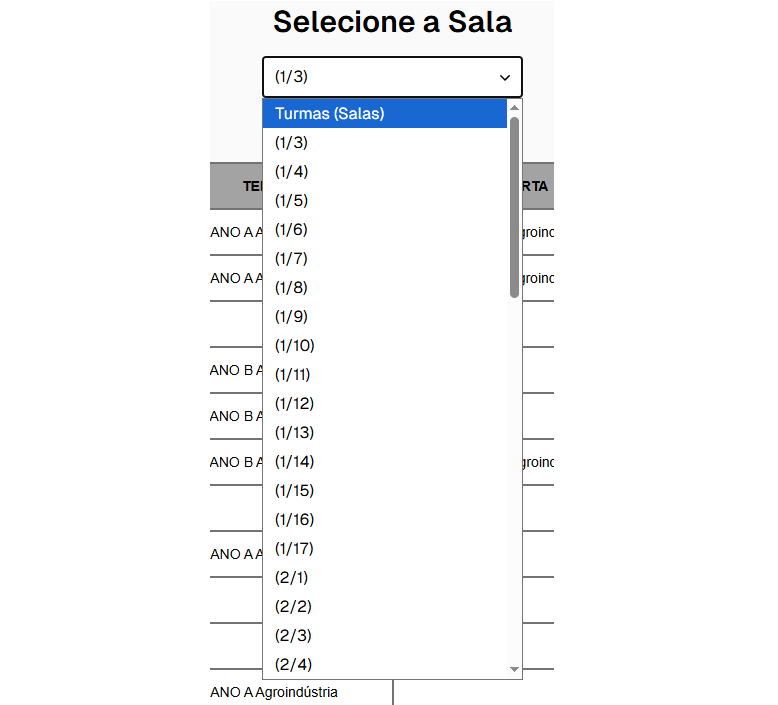
\includegraphics[width=0.3\textwidth]{Figuras/front-19.png}
        \caption*{Fonte: AUTOR (2025)}
        \label{fig_front_19}
    \end{figure}
    
    \item Download em pdf: permite exportar e salvar as tabelas de horários no formato PDF, facilitando o acesso offline. A seguir, será mostrado na Figura \ref{fig_front_20}.

    \begin{figure}[htb]
        \centering
        \caption{Download em pdf}
        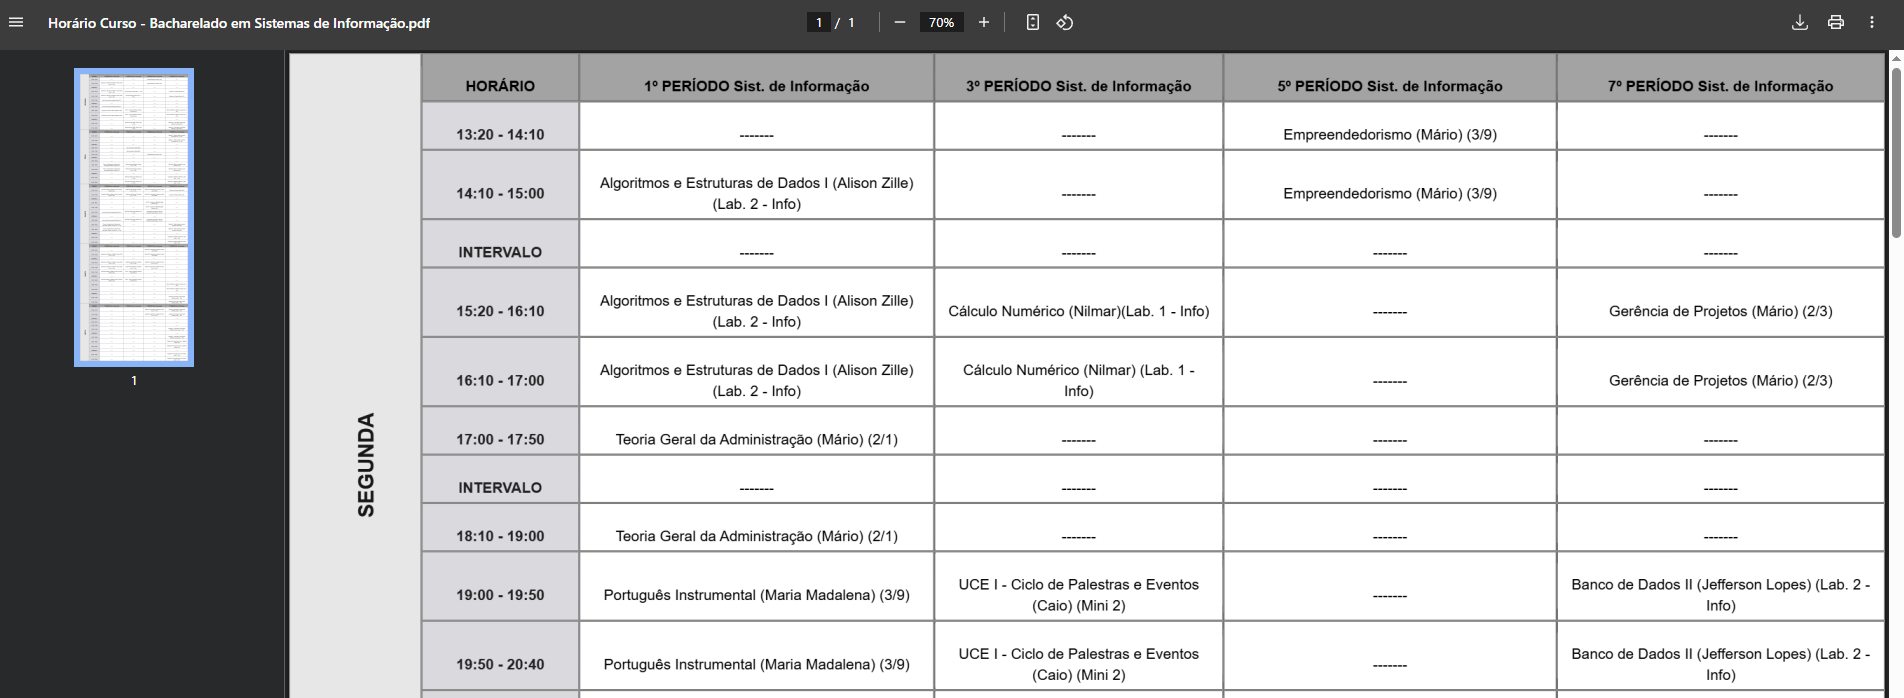
\includegraphics[width=0.8\textwidth]{Figuras/front-20.png}
        \caption*{Fonte: AUTOR (2025)}
        \label{fig_front_20}
    \end{figure}
    
    \item Tela de Login: restringe o acesso à tela de validação de dados apenas aos administradores, por meio de autenticação com usuário e senha. Ver Figura \ref{fig_front_21}.

    \begin{figure}[htb]
        \centering
        \caption{Tela de login com credenciais incorretas}
        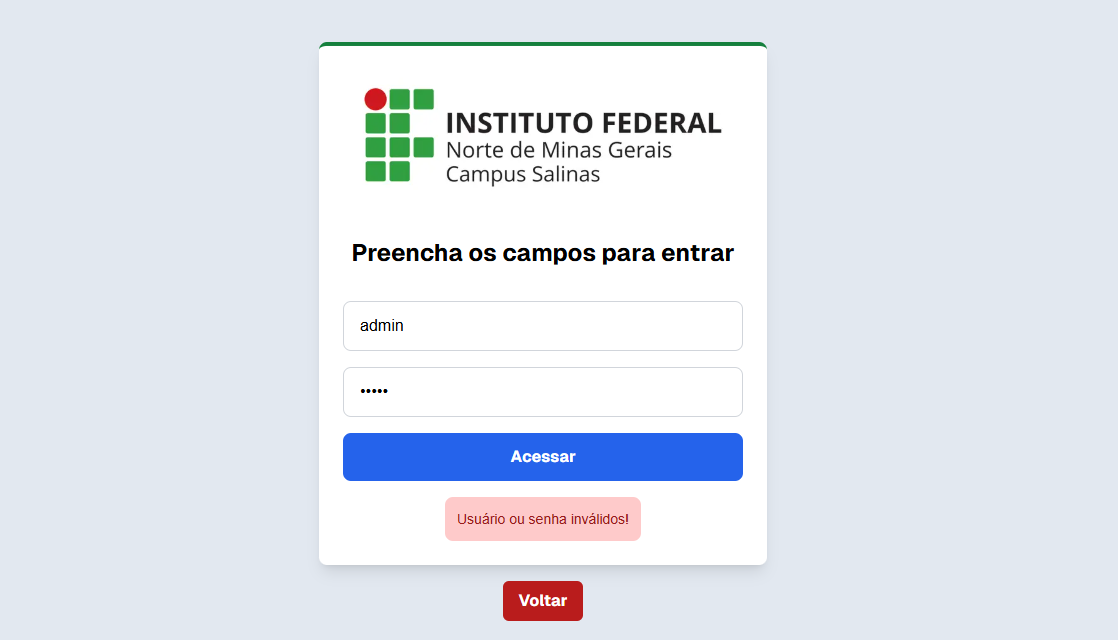
\includegraphics[width=0.8\textwidth]{Figuras/front-21.png}
        \caption*{Fonte: AUTOR (2025)}
        \label{fig_front_21}
    \end{figure}
    
    \item Tela de validação: exibe os resultados da verificação da planilha de horários, apresentando uma tabela com indicadores de conformidade (SIM ou NÃO) e validando:
    \begin{itemize}
        \item a presença das guias Horário - Ensino Médio, Horário - Graduação e Validação de Dados;
        \item a existência dos intervalos de células (B2:V76), (B2:AW106) e (A2:A);
        \item a formatação correta dos nomes, verificando se contêm os parênteses exigidos para turmas e professores. Se forem encontradas inconsistências, a tela exibe as células problemáticas, informando a guia, coluna e linha correspondentes. Ilustrado na Figura \ref{fig_front_22}.
    \end{itemize}

    \begin{figure}[htb]
        \centering
        \caption{Tela de Validação com resultados}
        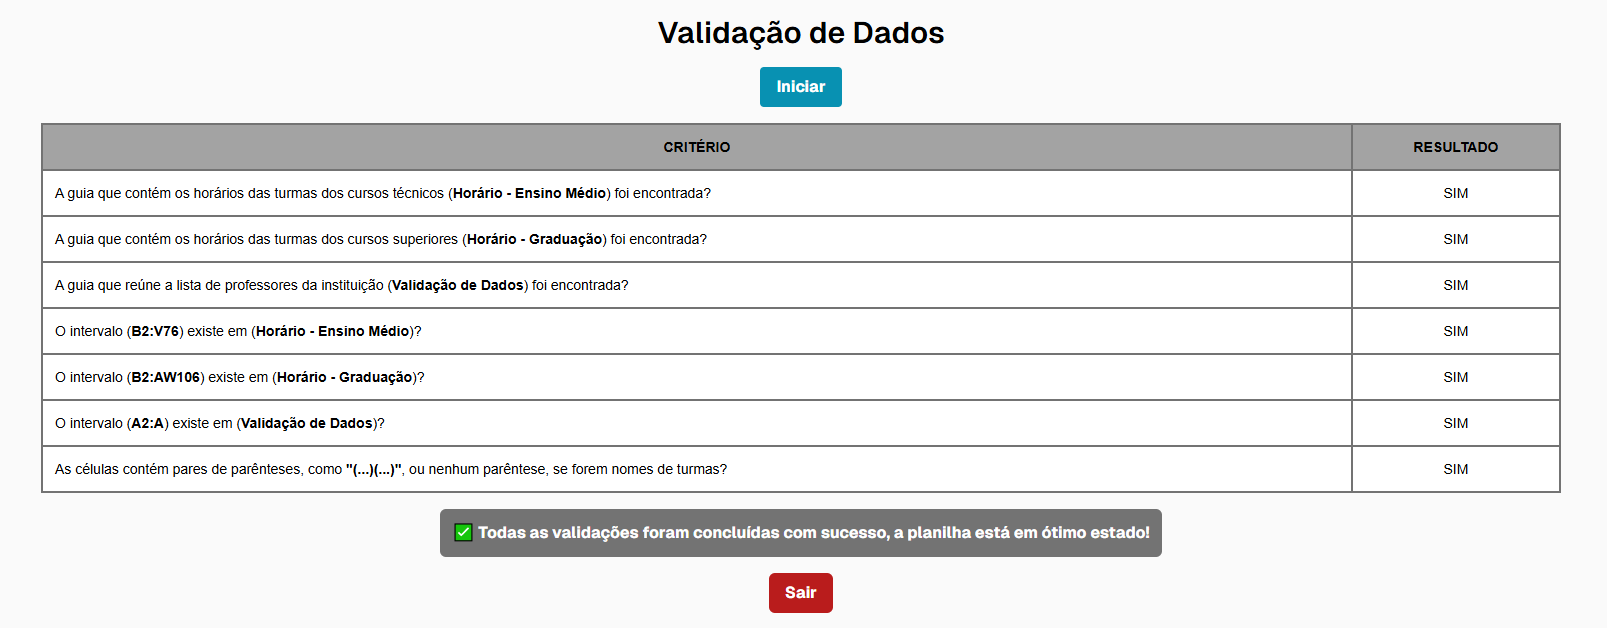
\includegraphics[width=1\textwidth]{Figuras/front-22.png}
        \caption*{Fonte: AUTOR (2025)}
        \label{fig_front_22}
    \end{figure}
\end{itemize}

\section{Back-end}

\subsection{Google Sheets como Banco de Dados}

As Figuras \ref{fig_plan_1}, \ref{fig_plan_2}, e \ref{fig_plan_3} apresentam as guias com a estrutura vital para o correto funcionamento do sistema, contendo os horários acadêmicos e a lista de professores disponíveis.

\begin{figure}[htb]
    \centering
    \caption{Horário - Ensino Médio}
    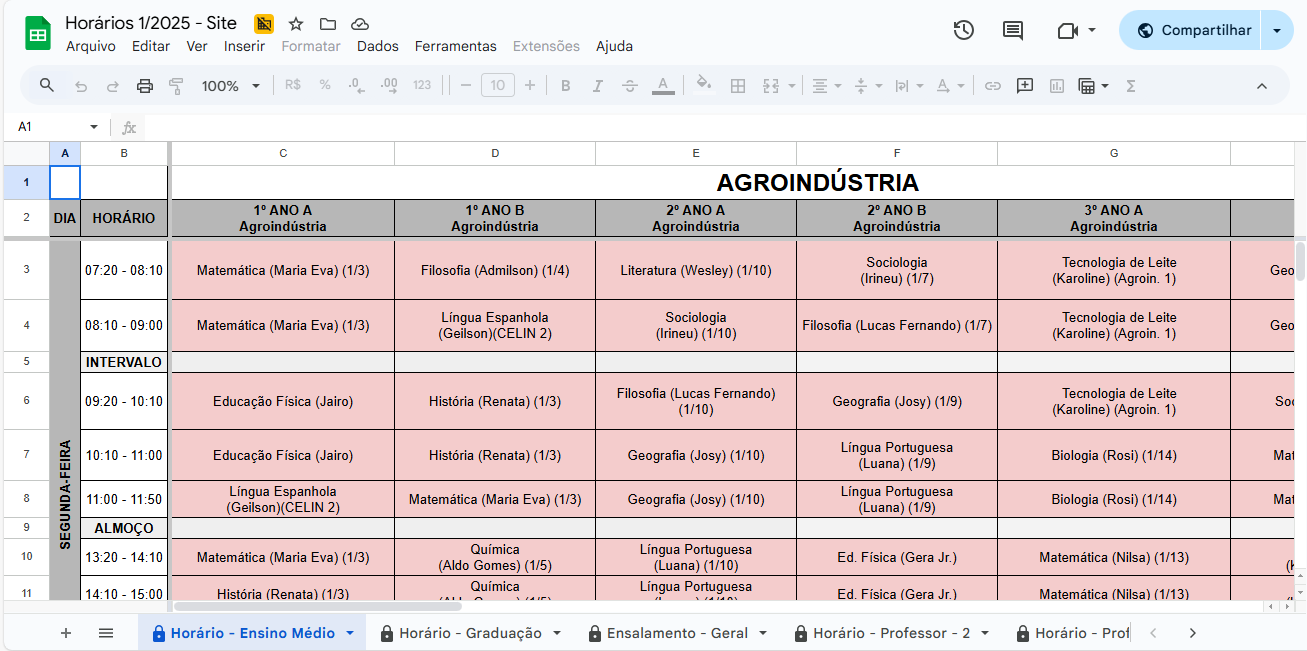
\includegraphics[width=0.9\textwidth]{Figuras/plan-1.png}
    \caption*{Fonte: AUTOR (2025)}
    \label{fig_plan_1}
\end{figure}

\begin{itemize}
    \item \textbf{Intervalo de células}: B2:V76
    \item \textbf{Descrição}: Contém os horários das turmas dos cursos técnicos.
\end{itemize}

\begin{figure}[htb]
    \centering
    \caption{Horário - Graduação}
    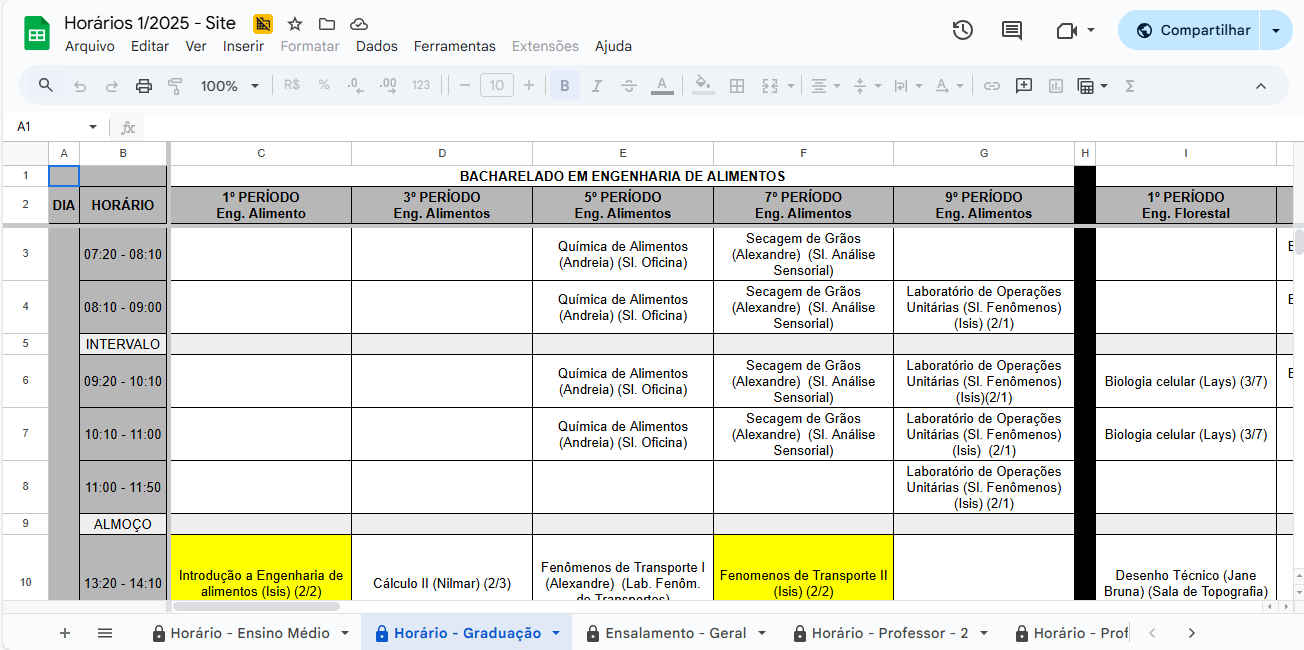
\includegraphics[width=0.9\textwidth]{Figuras/plan-2.png}
    \caption*{Fonte: AUTOR (2025)}
    \label{fig_plan_2}
\end{figure}

\begin{itemize}
    \item \textbf{Intervalo de células}: B2:AW106
    \item \textbf{Descrição}: Contém os horários das turmas dos cursos superiores.
\end{itemize}

\begin{figure}[htb]
    \centering
    \caption{Validação de Dados}
    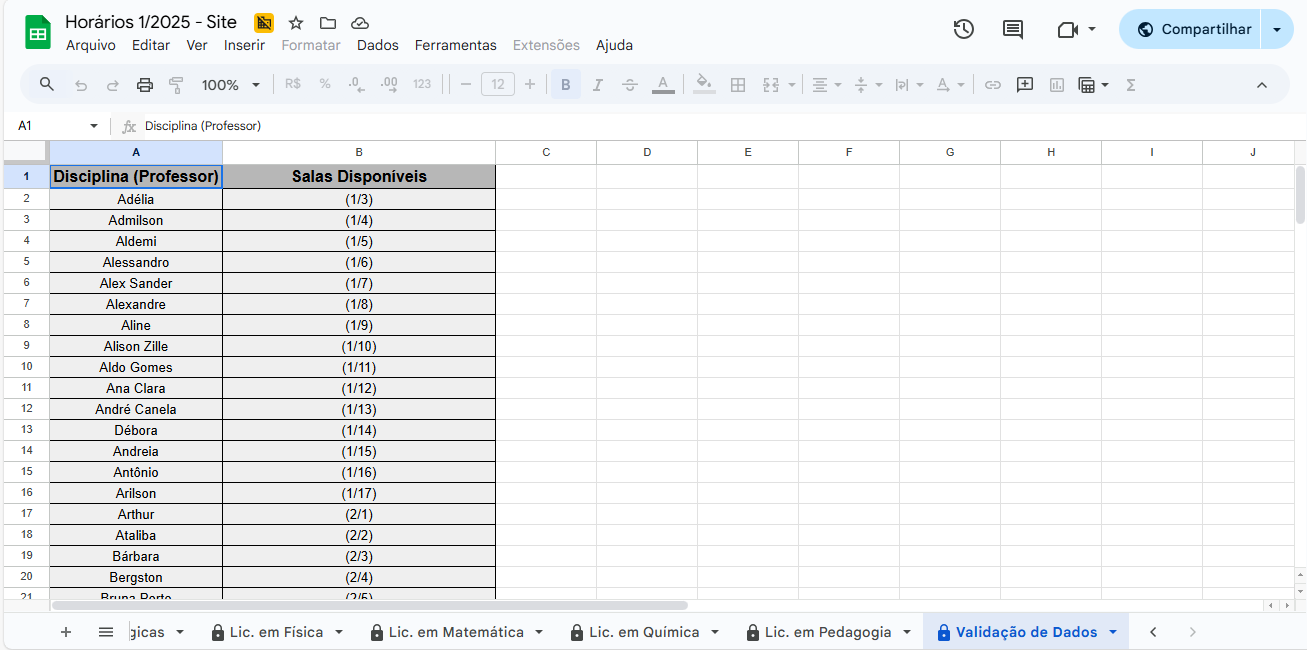
\includegraphics[width=0.9\textwidth]{Figuras/plan-3.png}
    \caption*{Fonte: AUTOR (2025)}
    \label{fig_plan_3}
\end{figure}

\begin{itemize}
    \item \textbf{Intervalo de células}: A2:A
    \item \textbf{Descrição}: Reúne a lista de professores da instituição.
\end{itemize}

A Figura \ref{fig_plan_4} apresenta a guia da planilha com as credenciais de login para acessar a tela de validação de dados:

\begin{figure}[htb]
    \centering
    \caption{Login}
    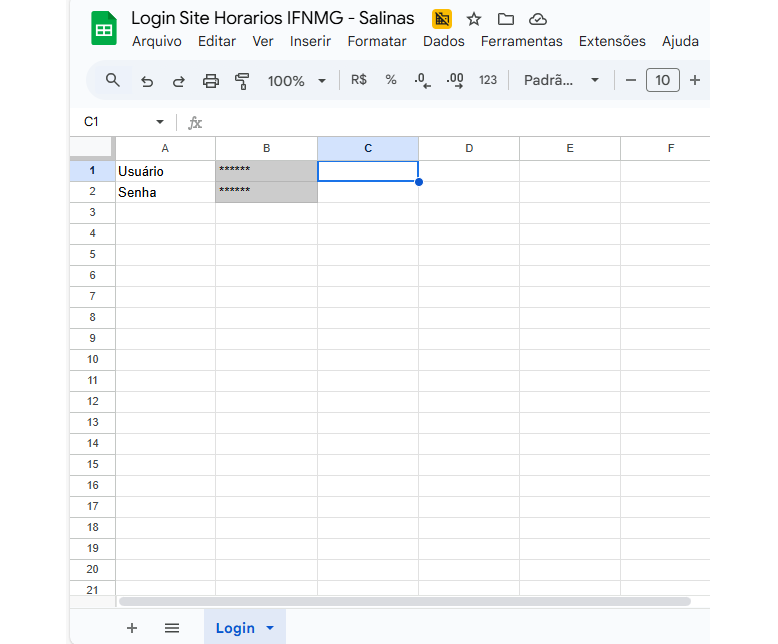
\includegraphics[width=0.9\textwidth]{Figuras/plan-4.png}
    \caption*{Fonte: AUTOR (2025)}
    \label{fig_plan_4}
\end{figure}

\begin{itemize}
    \item \textbf{Intervalo de células}: B1:B2
    \item \textbf{Descrição}: Contém as credenciais de usuário e senha para acessar a tela de validação de dados.
\end{itemize}

\subsection{Desenvolvimento do Back-end}

O back-end foi desenvolvido utilizando o framework Spring Boot, escolhido por sua robustez, flexibilidade e ampla adoção no mercado. Essa tecnologia possibilitou integrar de forma segura a API do Google Sheets, garantindo a leitura dos dados necessários para o funcionamento da plataforma e enviando essas informações ao front-end de maneira estruturada e confiável. Todo o processo priorizou simplicidade na configuração e facilidade de manutenção, permitindo atender às demandas do projeto com agilidade. O código está disponível no repositório do projeto em \url{https://github.com/Tomaz5556/Horarios-IFNMG-Salinas}.

\subsection{Estrutura do Back-end}

A estrutura do back-end está organizada seguindo o padrão arquitetural MVC, o que favorece a separação de responsabilidades, facilita a manutenção e a evolução do sistema. Na Figura \ref{fig_back_1}, destacam-se os principais elementos do projeto:

\begin{figure}[htb]
    \centering
    \caption{Estrutura do back-end}
    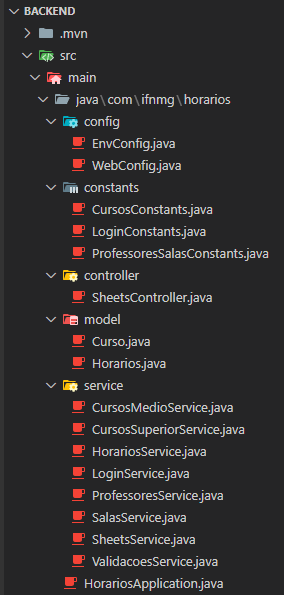
\includegraphics[width=0.4\textwidth]{Figuras/back-1.png}
    \caption*{Fonte: AUTOR (2025)}
    \label{fig_back_1}
\end{figure}

\begin{itemize}
    \item config: pasta responsável por armazenar classes de configuração do sistema, incluindo a EnvConfig.java, que define as variáveis de ambiente, e a WebConfig.java, responsável pelos ajustes de configuração da aplicação Spring Boot.
    \item constants: pasta responsável por centralizar valores fixos e listas utilizadas no sistema, contendo as classes CursosConstants.java, LoginConstants.java e ProfessoresSalasConstants.java, que mantêm os dados de cursos, professores, salas e credenciais de login.
    \item controller: pasta responsável por controlar as requisições recebidas e encaminhá-las para os serviços adequados, abrigando a classe SheetsController.java, que gerencia as rotas da aplicação.
    \item model: pasta responsável por definir as classes de domínio que representam a estrutura dos dados, como Curso.java e Horarios.java, que servem de modelo para a manipulação das informações obtidas do Google Sheets.
    \item service: pasta responsável por concentrar as regras de negócio e a comunicação com a API do Google Sheets, incluindo as classes CursosMedioService.java, CursosSuperiorService.java, HorariosService.java, LoginService.java, ProfessoresService.java, SalasService.java, SheetsService.java e ValidacoesService.java.
    \item HorariosApplication.java: arquivo inicializador da aplicação Spring Boot, responsável por executar o sistema e carregar todas as configurações necessárias para o funcionamento da plataforma.
\end{itemize}

\subsection{Funcionalidades do Back-end}

\begin{itemize}
    \item Estabelecer a conexão segura com a API do Google Sheets para coletar os dados das planilhas utilizadas como banco de dados da aplicação. A seguir, será mostrado na Figura \ref{fig_back_2}.
    
    \begin{figure}[H]
        \centering
        \caption{SheetsService.java}
        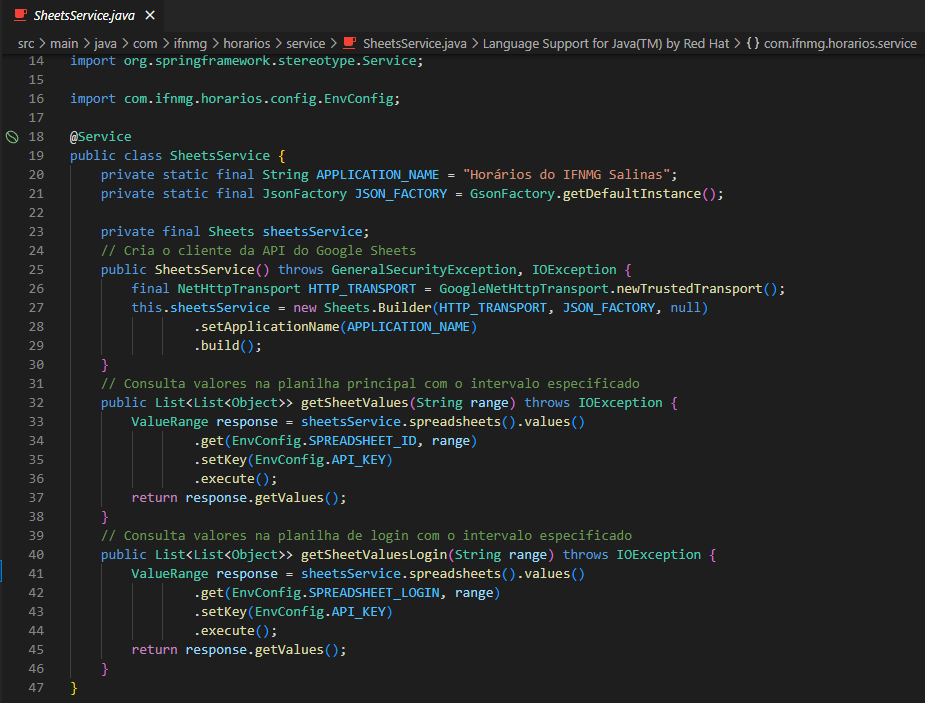
\includegraphics[width=1\textwidth]{Figuras/back-2.png}
        \caption*{Fonte: AUTOR (2025)}
        \label{fig_back_2}
    \end{figure}

    \item Disponibilizar endpoints REST para consulta de horários de cursos, professores, salas e resultados de validação de dados, assegurando respostas padronizadas e consistentes. Apresentado na Figura \ref{fig_back_3}.
    
    \begin{figure}[H]
        \centering
        \caption{SheetsController.java}
        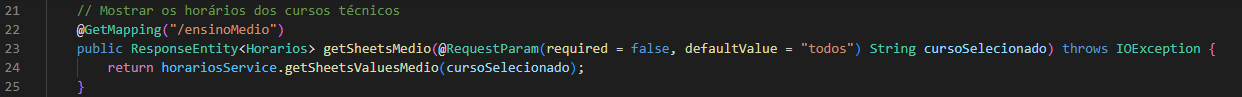
\includegraphics[width=1\textwidth]{Figuras/back-3.png}
        \caption*{Fonte: AUTOR (2025)}
        \label{fig_back_3}
    \end{figure}
\end{itemize}

\section{Deploy}

O front-end foi hospedado na plataforma Vercel, permitindo a disponibilização da interface do usuário com alta performance e integração contínua, como mostrado na Figura \ref{fig_deploy_1}.

\begin{figure}[htb]
    \centering
    \caption{Deploy do front-end da plataforma na Vercel}
    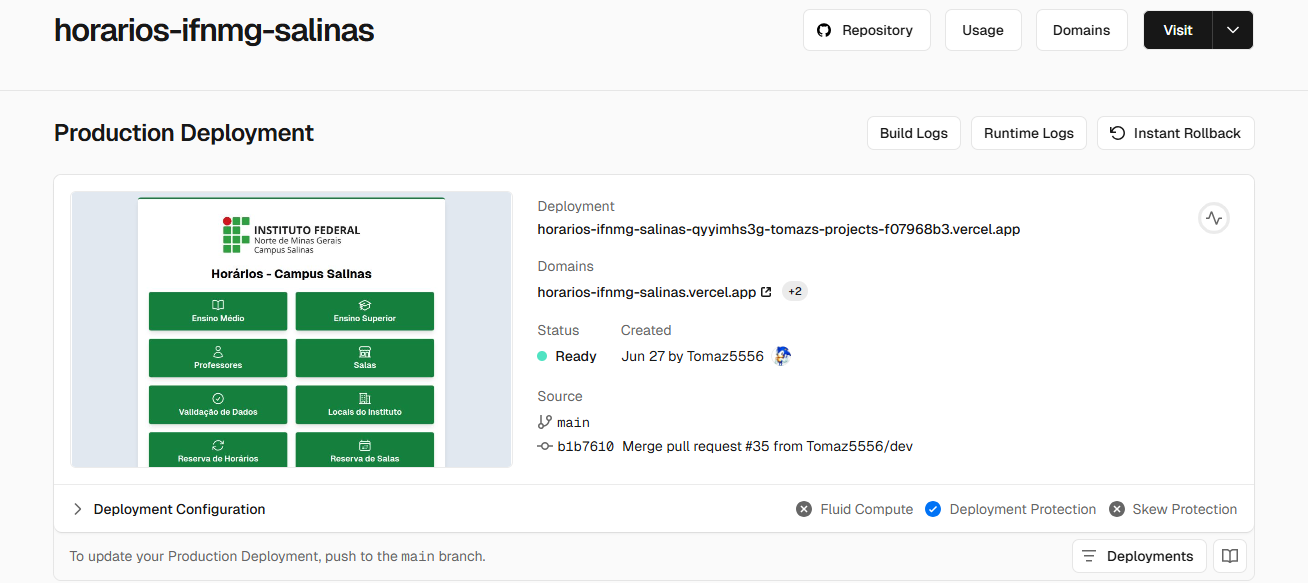
\includegraphics[width=1\textwidth]{Figuras/deploy-1.png}
    \caption*{Fonte: AUTOR (2025)}
    \label{fig_deploy_1}
\end{figure}

Já o back-end foi hospedado na plataforma Koyeb, responsável por executar a API que processa e envia os dados do Google Sheets ao front-end, conforme ilustrado na Figura \ref{fig_deploy_2}.

\begin{figure}[htb]
    \centering
    \caption{Deploy do back-end da plataforma na Koyeb}
    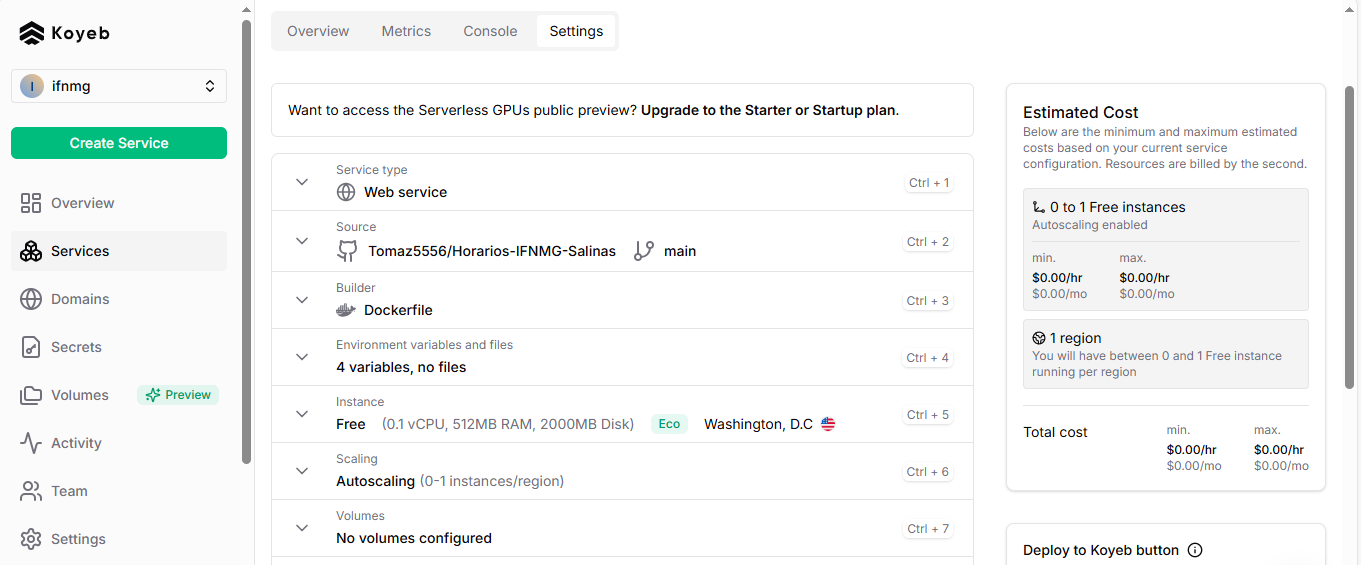
\includegraphics[width=1\textwidth]{Figuras/deploy-2.png}
    \caption*{Fonte: AUTOR (2025)}
    \label{fig_deploy_2}
\end{figure}

\section{Documentação}

As Figuras \ref{fig_doc_1}, \ref{fig_doc_2} e \ref{fig_doc_3} apresentam a documentação técnica elaborada para a planilha utilizada como banco de dados do sistema. A documentação está disponível no repositório do projeto, no endereço \url{https://tomaz5556.github.io/Horarios-IFNMG-Salinas}. Esse material descreve de forma clara e objetiva as instruções para atualização do identificador da planilha, as regras de preenchimento dos dados e os padrões de nomes e intervalos de células necessários para garantir a integridade do funcionamento da plataforma.

\begin{figure}[H]
    \centering
    \caption{Instruções para desenvolvedores}
    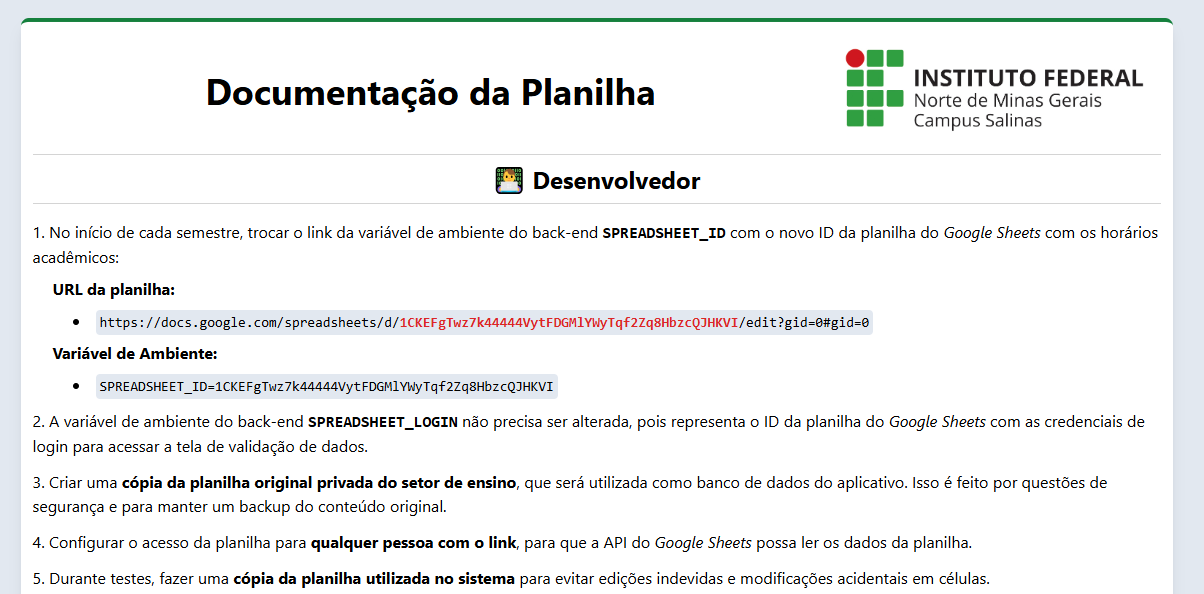
\includegraphics[width=1\textwidth]{Figuras/doc-1.png}
    \caption*{Fonte: AUTOR (2025)}
    \label{fig_doc_1}
\end{figure}

\begin{figure}[htb]
    \centering
    \caption{Instruções para administradores da planilha}
    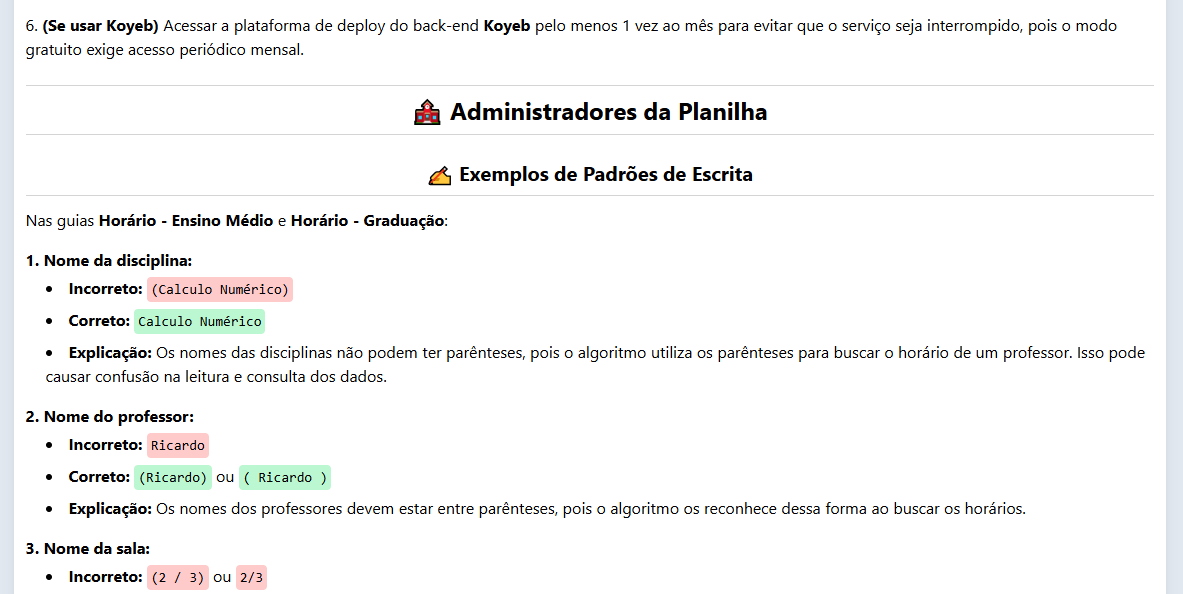
\includegraphics[width=1\textwidth]{Figuras/doc-2.png}
    \caption*{Fonte: AUTOR (2025)}
    \label{fig_doc_2}
\end{figure}

\begin{figure}[htb]
    \centering
    \caption{Explicação das guias e intervalos de células}
    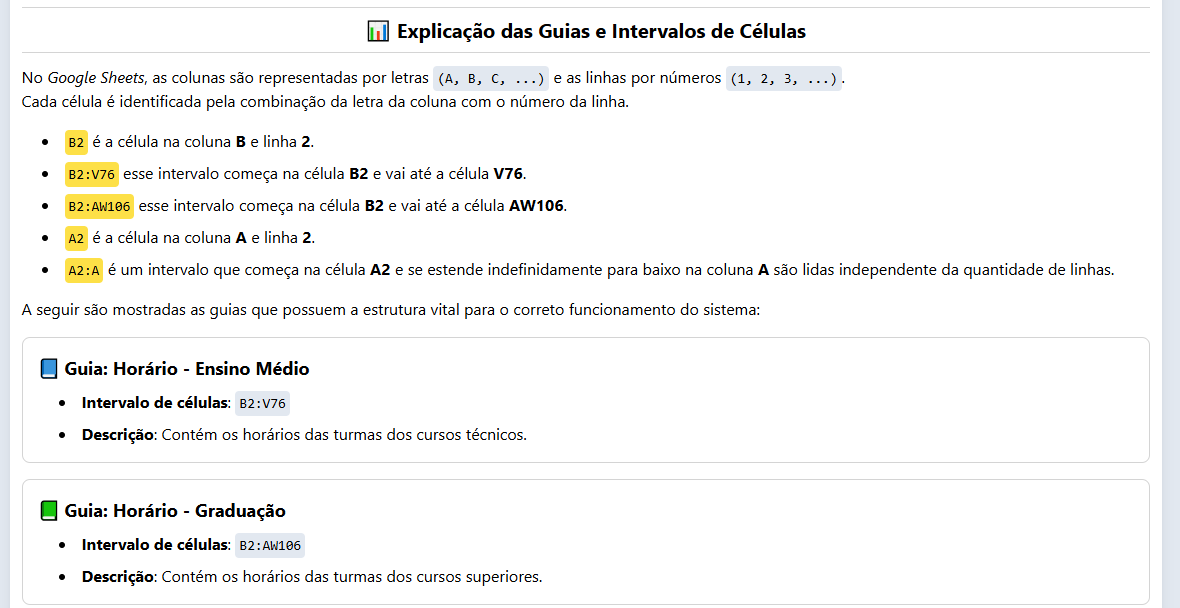
\includegraphics[width=1\textwidth]{Figuras/doc-3.png}
    \caption*{Fonte: AUTOR (2025)}
    \label{fig_doc_3}
\end{figure}

\begin{figure}[htb]
    \centering
    \caption{Observação sobre mudanças estruturais}
    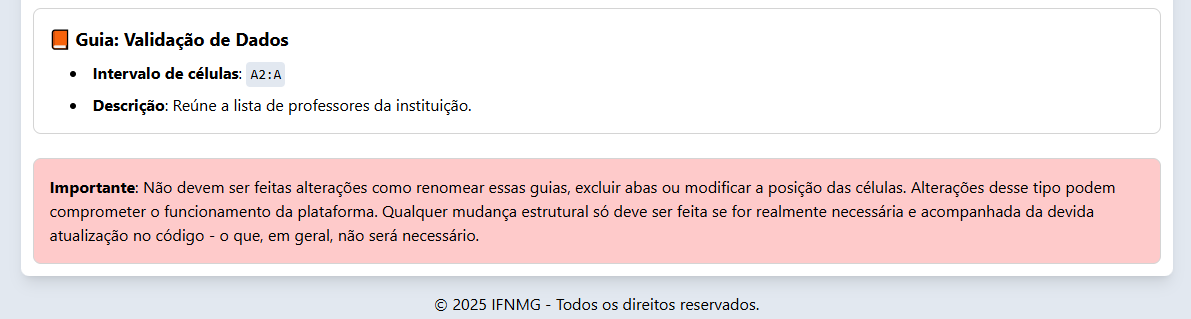
\includegraphics[width=1\textwidth]{Figuras/doc-4.png}
    \caption*{Fonte: AUTOR (2025)}
    \label{fig_doc_4}
\end{figure}